%!TeX root=../viewsbodytop.tex
\addchap{The Undignified Melodrama of the Bone of Contention}

\lettrine[lines=4,ante=‘]{I}{} am afraid you have brought shocking weather with you, Lord~Peter,' said Mrs~Frobisher-Pym, with playful reproof. »If it goes on like this they will have a bad day for the funeral.«

\zz
Lord~Peter Wimsey glanced out of the morning-room window to the soaked green lawn and the shrubbery, where the rain streamed down remorselessly over the laurel leaves, stiff and shiny like mackintoshes.

»Nasty exposed business, standing round at funerals,« he agreed.

»Yes, I always think it's such a shame for the old people. In a tiny village like this it's about the only pleasure they get during the winter. It makes something for them to talk about for weeks.«

»Is it anybody's funeral in particular?«

»My dear Wimsey,« said his host, »it is plain that you, coming from your little village of London, are quite out of the swim. There has never been a funeral like it in Little Doddering before. It's an event.«

»Really?«

»Oh dear, yes. You may possibly remember old Burdock?«

»Burdock? Let me see. Isn't he a sort of local squire, or something?«

»He was,« corrected Mr~Frobisher-Pym. »He's dead—died in New York about three weeks ago, and they're sending him over to be buried. The Burdocks have lived in the big house for hundreds of years, and they're all buried in the churchyard, except, of course, the one who was killed in the War. Burdock's secretary cabled the news of his death across, and said the body was following as soon as the embalmers had finished with it. The boat gets in to Southampton this morning, I believe. At any rate, the body will arrive here by the 6.30 from Town.«

»Are you going down to meet it, Tom?«

»No, my dear. I don't think that is called for. There will be a grand turn-out of the village, of course. Joliffe's people are having the time of their lives; they borrowed an extra pair of horses from young Mortimer for the occasion. I only hope they don't kick over the traces and upset the hearse. Mortimer's horseflesh is generally on the spirited side.«

»But, Tom, we must show some respect to the Burdocks.«

»We're attending the funeral to-morrow, and that's quite enough. We must do that, I suppose, out of consideration for the family, though, as far as the old man himself goes, respect is the very last thing anybody would think of paying him.«

»Oh, Tom, he's dead.«

»And quite time too. No, Agatha, it's no use pretending that old Burdock was anything but a spiteful, bad-tempered, dirty-living old blackguard that the world's well rid of. The last scandal he stirred up made the place too hot to hold him. He had to leave the country and go to the States, and, even so, if he hadn't had the money to pay the people off, he'd probably have been put in gaol. That's why I'm so annoyed with Hancock. I don't mind his calling himself a priest, though clergyman was always good enough for dear old Weeks—who, after all, was a canon—and I don't mind his vestments. He can wrap himself up in a Union Jack if he likes—it doesn't worry \textit{me}. But when it comes to having old Burdock put on trestles in the south aisle, with candles round him, and Hubbard from the »Red Cow« and Duggins's boy praying over him half the night, I think it's time to draw the line. The people don't like it, you know—as least, the older generation don't. It's all right for the young ones, I dare say; they must have their amusement; but it gives offence to a lot of the farmers. After all, they knew Burdock a bit too well. Simpson—he's people's warden, you know—came up quite in distress to speak to me about it last night. You couldn't have a sounder man than Simpson. I said I would speak to Hancock. I did speak to him this morning, as a matter of fact, but you might as well talk to the west door of the church.«

»Mr~Hancock is one of those young men who fancy they know everything,« said his wife. »A sensible man would have listened to you, Tom. You're a magistrate and have lived here all your life, and it stands to reason you know considerably more about the parish than he does.«

»He took up the ridiculous position,« said Mr~Frobisher-Pym, »that the more sinful the old man had been the more he needed praying for. I said, »I think it would need more praying than you or I could do to help old Burdock out of the place he's in now.« Ha, ha! So he said, »I agree with you, Mr~Frobisher-Pym; that is why I am having eight watchers to pray all through the night for him.« I admit he had me there.«

»Eight people?« exclaimed Mrs~Frobisher-Pym.

»Not all at once, I understand; in relays, two at a time. »Well,« I said, »I think you ought to consider that you will be giving a handle to the Nonconformists.« Of course, he couldn't deny that.«

Wimsey helped himself to marmalade. Nonconformists, it seemed, were always searching for handles. Though what kind—whether door-handles, tea-pot handles, pump-handles, or starting-handles—was never explained, nor what the handles were to be used for when found. However, having been brought up in the odour of the Establishment, he was familiar with this odd dissenting peculiarity, and merely said:

»Pity to be extreme in a small parish like this. Disturbs the ideas of the simple fathers of the hamlet and the village blacksmith, with his daughter singin' in the choir and the Old Hundredth and all the rest of it. Don't Burdock's family have anything to say to it? There are some sons, aren't there?«

»Only the two, now. Aldine was the one that was killed, of course, and Martin is somewhere abroad. He went off after that row with his father, and I don't think he has been back in England since.«

»What was the row about?«

»Oh, that was a disgraceful business. Martin got a girl into trouble—a film actress or a typist or somebody of that sort—and insisted on marrying her.«

»Oh?«

»Yes, so dreadful of him,« said the lady, taking up the tale, »when he was practically engaged to the Delaprime girl—the one with glasses, you know. It made a terrible scandal. Some horribly vulgar people came down and pushed their way into the house and insisted on seeing old Mr~Burdock. I will say for him he stood up to them—he wasn't the sort of person you could intimidate. He told them the girl had only herself to blame, and they could sue Martin if they liked—\textit{he} wouldn't be blackmailed on his son's account. The butler was listening at the door, naturally, and told the whole village about it. And then Martin Burdock came home and had a quarrel with his father you could have heard for miles. He said that the whole thing was a lie, and that he meant to marry the girl, anyway. I cannot understand how anybody could marry into a blackmailing family like that.«

»My dear,« said Mr~Frobisher-Pym gently, »I don't think you're being quite fair to Martin, or his wife's parents, either. From what Martin told me, they were quite decent people, only not his class, of course, and they came in a well-meaning way to find out what Martin's »intentions« were. You would want to do the same yourself, if it were a daughter of ours. Old Burdock, naturally, thought they meant blackmail. He was the kind of man who thinks everything can be paid for; and he considered a son of his had a perfect right to seduce a young woman who worked for a living. I don't say Martin was altogether in the right\longdash«

»Martin is a chip off the old block, I'm afraid,« retorted the lady. »He married the girl, anyway, and why should he do that, unless he had to?«

»Well, they've never had any children, you know,« said Mr~Frobisher-Pym.

»That's as may be. I've no doubt the girl was in league with her parents. And you know the Martin Burdocks have lived in Paris ever since.«

»That's true,« admitted her husband. »It was an unfortunate affair altogether. They've had some difficulty in tracing Martin's address, too, but no doubt he'll be coming back shortly. He is engaged in producing some film play, they tell me, so possibly he can't get away in time for the funeral.«

»If he had any natural feeling, he would not let a film play stand in his way,« said Mrs~Frobisher-Pym.

»My dear, there are such things as contracts, with very heavy monetary penalties for breaking them. And I don't suppose Martin could afford to lose a big sum of money. It's not likely that his father will have left him anything.«

»Martin is the younger son, then?« asked Wimsey, politely showing more interest than he felt in the rather well-worn plot of this village melodrama.

»No, he is the eldest of the lot. The house is entailed, of course, and so is the estate, such as it is. But there's no money in the land. Old Burdock made his fortune in rubber shares during the boom, and the money will go as he leaves it—wherever that may be, for they haven't found any will yet. He's probably left it all to Haviland.«

»The younger son?«

»Yes. He's something in the City—a director of a company—connected with silk stockings, I believe. Nobody has seen very much of him. He came down as soon as he heard of his father's death. He's staying with the Hancocks. The big house has been shut up since old Burdock went to the States four years ago. I suppose Haviland thought it wasn't worth while opening it up till they knew what Martin was going to do about it. That's why the body is being taken to the church.«

»Much less trouble, certainly,« said Wimsey.

»Oh, yes—though, mind you, I think Haviland ought to take a more neighbourly view of it. Considering the position the Burdocks have always held in the place, the people had a right to expect a proper reception after the funeral. It's usual. But these business people think less of tradition than we do down here. And, naturally, since the Hancocks are putting Haviland up, he can't raise much objection to the candles and the prayers and things.«

»Perhaps not,« said Mrs~Frobisher-Pym, »but it would have been more suitable if Haviland had come to us, rather than to the Hancocks, whom he doesn't even know.«

»My dear, you forget the very unpleasant dispute I had with Haviland Burdock about shooting over my land. After the correspondence that passed between us, last time he was down here, I could scarcely offer him hospitality. His father took a perfectly proper view of it, I will say that for him, but Haviland was exceedingly discourteous to me, and things were said which I could not possibly overlook. However, we mustn't bore you, Lord~Peter, with our local small-talk. If you've finished your breakfast, what do you say to a walk round the place? It's a pity it's raining so hard—and you don't see the garden at its best this time of the year, of course—but I've got some cocker span'els you might like to have a look at.«

Lord~Peter expressed eager anxiety to see the spaniels, and in a few minutes' time found himself squelching down the gravel path which led to the kennels.

»Nothing like a healthy country life,« said Mr~Frobisher-Pym. »I always think London is so depressing in the winter. Nothing to do with one's self. All right to run up for a day or two and see a theatre now and again, but how you people stick it week in and week out beats me. I must speak to Plunkett about this archway,« he added. »It's getting out of trim.«

He broke off a dangling branch of ivy as he spoke. The plant shuddered revengefully, tipping a small shower of water down Wimsey's neck.

The cocker spaniel and her family occupied a comfortable and airy stall in the stable buildings. A youngish man in breeches and leggings emerged to greet the visitors, and produced the little bundles of puppy-hood for their inspection. Wimsey sat down on an upturned bucket and examined them gravely one by one. The bitch, after cautiously reviewing his boots and grumbling a little, decided that he was trustworthy and slobbered genially over his knees.

»Let me see,« said Mr~Frobisher-Pym, »how old are they?«

»Thirteen days, sir.«

»Is she feeding them all right?«

»Fine, sir. She's having some of the malt food. Seems to suit her very well, sir.«

»Ah, yes. Plunkett was a little doubtful about it, but I heard it spoken very well of. Plunkett doesn't care for experiments, and, in a general way, I agree with him. Where is Plunkett, by the way?«

»He's not very well this morning, sir.«

»Sorry to hear that, Merridew. The rheumatics again?«

»No, sir. From what Mrs~Plunkett tells me, he's had a bit of a shock.«

»A shock? What sort of a shock? Nothing wrong with Alf or Elsie, I hope?«

»No, sir. The fact is—I understand he's seen something, sir.«

»What do you mean, seen something?«

»Well, sir—something in the nature of a warning, from what he says.«

»A warning? Good heavens, Merridew, he mustn't get those sort of ideas in his head. I'm surprised at Plunkett; I always thought he was a very level-headed man. What sort of warning did he say it was?«

»I couldn't say, sir.«

»Surely he mentioned what he thought he'd seen.«

Merridew's face took on a slightly obstinate look.

»I can't say, I'm sure, sir.«

»This will never do. I must go and see Plunkett. Is he at the cottage?«

»Yes, sir.«

»We'll go down there at once. You don't mind, do you, Wimsey? I can't allow Plunkett to make himself ill. If he's had a shock he'd better see a doctor. Well, carry on, Merridew, and be sure you keep her warm and comfortable. The damp is apt to come up through these brick floors. I'm thinking of having the whole place re-set with concrete, but it takes money, of course. I can't imagine,« he went on, as he led the way past the greenhouse towards a trim cottage set in its own square of kitchen-garden, »what can have happened to have upset Plunkett. I hope it's nothing serious. He's getting elderly, of course, but he ought to be above believing in warnings. You wouldn't believe the extraordinary ideas these people get hold of. Fact is, I expect he's been round at the »Weary Traveller,« and caught sight of somebody's washing hung out on the way home.«

»Not washing,« corrected Wimsey mechanically. He had a deductive turn of mind which exposed the folly of the suggestion even while irritably admitting that the matter was of no importance. »It poured with rain last night, and, besides, it's Thursday. But Tuesday and Wednesday were fine, so the drying would have all been done then. No washing.«

»Well, well—something else then—a post, or old Mrs~Giddens's white donkey. Plunkett does occasionally take a drop too much, I'm sorry to say, but he's a very good kennel-man, so one overlooks it. They're superstitious round about these parts, and they can tell some queer tales if once you get into their confidence. You'd be surprised how far off the main track we are as regards civilisation. Why, not here, but at Abbotts Bolton, fifteen miles off, it's as much as one's life's worth to shoot a hare. Witches, you know, and that sort of thing.«

»I shouldn't be a bit surprised. They'll still tell you about werewolves in some parts of Germany.«

»Yes, I dare say. Well, here we are.« Mr~Frobisher-Pym rapped loudly with his walking-stick on the door of the cottage and turned the handle without waiting for permission.

»You there, Mrs~Plunkett? May we come in? Ah! good morning. Hope we're not disturbing you, but Merridew told me Plunkett was not so well. This is Lord~Peter Wimsey—a very old friend of mine; that is to say, I'm a very old friend of \textit{his}; ha, ha!«

»Good morning, sir; good morning, your lordship. I'm sure Plunkett will be very pleased to see you. Please step in. Plunkett, here's Mr~Pym to see you.«

The elderly man who sat crouching over the fire turned a mournful face towards them, and half rose, touching his forehead.

»Well, now, Plunkett, what's the trouble?« enquired Mr~Frobisher-Pym, with the hearty bedside manner adopted by country gentlefolk visiting their dependants. »Sorry not to see you out and about. Touch of the old complaint, eh?«

»No, sir; no, sir. Thank you, sir. I'm well enough in myself. But I've had a warning, and I'm not long for this world.«

»Not long for this world? Oh, nonsense, Plunkett. You mustn't talk like that. A touch of indigestion, that's what you've got, I expect. Gives one the blues, I know. I'm sure I often feel like nothing on earth when I've got one of my bilious attacks. Try a dose of castor-oil, or a good old-fashioned blue pill and black draught. Nothing like it. Then you won't talk about warnings and dying.«

»No medicine won't do no good to \textit{my} complaint, sir. Nobody as see what I've seed ever got the better of it. But as you and the gentleman are here, sir, I'm wondering if you'll do me a favour.«

»Of course, Plunkett, anything you like. What is it?«

»Why, just to draw up my will, sir. Old Parson, he used to do it. But I don't fancy this new young man, with his candles and bits of things. It don't seem as if he'd make it good and legal, sir, and I wouldn't like it if there was any dispute after I was gone. So as there ain't much time left me, I'd be grateful if you'd put it down clear for me in pen and ink that I wants my little bit all to go to Sarah here, and after her to Alf and Elsie, divided up equal.«

»Of course I'll do that for you, Plunkett, any time you like. But it's all nonsense to be talking about wills. Bless my soul, I shouldn't be surprised if you were to see us all underground.«

»No, sir. I've been a hale and hearty man, I'm not denying. But I've been called, sir, and I've got to go. It must come to all of us, I know that. But it's a fearful thing to see the death-coach come for one, and know that the dead are in it, that cannot rest in the grave.«

»Come now, Plunkett, you don't mean to tell me you believe in that old foolishness about the death-coach. I thought you were an educated man. What would Alf say if he heard you talking such nonsense?«

»Ah, sir, young people don't know everything, and there's many more things in God's creation than what you'll find in the printed books.«

»Oh, well,« said Mr~Frobisher-Pym, finding this opening irresistible, »we know there are more things in heaven and earth, Horatio, than are dreamt of in your philosophy. Quite so. But that doesn't apply nowadays,« he added contradictorily. »There are no ghosts in the twentieth century. Just you think the matter out quietly, and you'll find you've made a mistake. There's probably some quite simple explanation. Dear me! I remember Mrs~Frobisher-Pym waking up one night and having a terrible fright, because she thought somebody'd been and hanged himself on our bedroom door. Such a silly idea, because I was safe in bed beside her—snoring, \textit{she} said, ha, ha!—and, if anybody was feeling like hanging himself, he wouldn't come into our bedroom to do it. Well, she clutched my arm in a great state of mind, and when I went to see what had alarmed her, what do you think it was? My trousers, which I'd hung up by the braces, with the socks still in the legs! My word! and didn't I get a wigging for not having put my things away tidy!«

Mr~Frobisher-Pym laughed, and Mrs~Plunkett said dutifully, »There now!« Her husband shook his head.

»That may be, sir, but I see the death-coach last night with my own eyes. Just striking midnight it was, by the church clock, and I see it come up the lane by the old priory wall.«

»And what were you doing out of bed at midnight, eh?«

»Well, sir, I'd been round to my sister's, that's got her boy home on leaf off of his ship.«

»And you'd been drinking his health, I dare say, Plunkett.« Mr~Frobisher-Pym wagged an admonitory forefinger.

»No, sir, I don't deny I'd had a glass or two of ale, but not to fuddle me. My wife can tell you I was sober enough when I got home.«

»That's right, sir. Plunkett hadn't taken too much last night, that I'll swear to.«

»Well, what was it you saw, Plunkett?«

»I see the death-coach, same as I'm telling you, sir. It come up the lane, all ghostly white, sir, and never making no more sound than the dead—which it were, sir.«

»A wagon or something going through to Lymptree or Herriotting.«

»No, sir—tweren't a wagon. I counted the horses—four white horses, and they went by with never a sound of hoof or bridle. And that weren't\longdash«

»Four horses! Come, Plunkett, you must have been seeing double. There's nobody about here would be driving four horses, unless it was Mr~Mortimer from Abbotts Bolton, and he wouldn't be taking his horseflesh out at midnight.«

»Four horses they was, sir. I see them plain. And it weren't Mr~Mortimer, neither, for he drives a drag, and this were a big, heavy coach, with no lights on it, but shinin' all of itself, with a colour like moonshine.«

»Oh, nonsense, man! You couldn't see the moon last night. It was pitch-dark.«

»No, sir, but the coach shone all moony-like, all the same.«

»And no lights? I wonder what the police would say to that.«

»No mortal police could stop that coach,« said Plunkett contemptuously, »nor no mortal man could abide the sight on it. I tell you, sir, that ain't the worst of it. The horses\longdash«

»Was it going slowly?«

»No, sir. It were going at a gallop, only the hoofs didn't touch the ground. There weren't no sound, and I see the black road and the white hoofs half a foot off of it. And the horses had no heads.«

»No heads?«

»No, sir.«

Mr~Frobisher-Pym laughed.

»Come, come, Plunkett, you don't expect us to swallow that. No heads? How could even a ghost drive horses with no heads? How about the reins, eh?«

»You may laugh, sir, but we know that with God all things are possible. Four white horses they was. I see them clearly, but there was neither head nor neck beyond the collar, sir. I see the reins, shining like silver, and they ran up to the rings of the hames, and they didn't go no further. If I was to drop down dead this minute, sir, that's what I see.«

»Was there a driver to this wonderful turn-out?«

»Yes, sir, there was a driver.«

»Headless too, I suppose?«

»Yes, sir, headless too. At least, I couldn't see nothing of him beyond his coat, which had them old-fashioned capes at the shoulders.«

»Well, I must say, Plunkett, you're very circumstantial. How far off was this—er—apparition when you saw it?«

»I was passing by the War Memorial, sir, when I see it come up the lane. It wouldn't be above twenty or thirty yards from where I stood. It went by at a gallop, and turned off to the left round the churchyard wall.«

»Well, well, it sounds odd, certainly, but it was a dark night, and at that distance your eyes may have deceived you. Now, if you'll take my advice you'll think no more about it.«

»Ah, sir, it's all very well saying that, but everybody knows the man who sees the death-coach of the Burdocks is doomed to die within the week. There's no use rebelling against it, sir; it is so. And if you'll be so good as to oblige me over that matter of a will, I'd die happier for knowing as Sarah and the children was sure of their bit of money.«

Mr~Frobisher-Pym obliged over the will, though much against the grain, exhorting and scolding as he wrote. Wimsey added his own signature as one of the witnesses, and contributed his own bit of comfort.

»I shouldn't worry too much about the coach, if I were you,« he said. »Depend upon it, if it's the Burdock coach it'll just have come for the soul of the old squire. It couldn't be expected to go to New York for him, don't you see? It's just gettin' ready for the funeral to-morrow.«

»That's likely enough,« agreed Plunkett. »Often and often it's been seen in these parts when one of the Burdocks was taken. But it's terrible unlucky to see it.«

The thought of the funeral seemed, however, to cheer him a little. The visitors again begged him not to think about it, and took their departure.

»Isn't it wonderful,« said Mr~Frobisher-Pym, »what imagination will do with these people? And they're obstinate. You could argue with them till you were black in the face.«

»Yes. I say, let's go down to the church and have a look at the place. I'd like to know how much he could really have seen from where he was standing.«

\begin{sidewaysfigure}
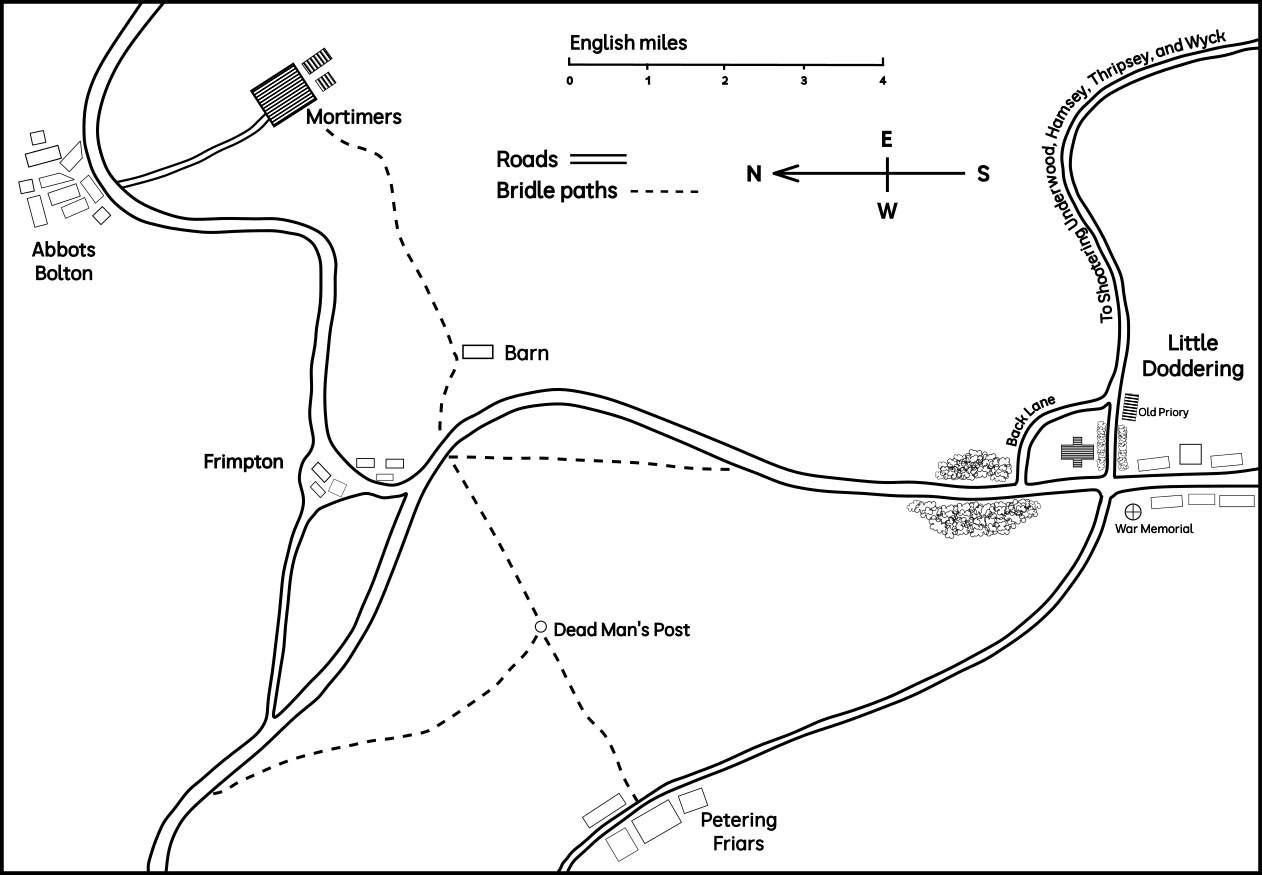
\includegraphics[width=\textwidth]{map}%
\end{sidewaysfigure}

%\begin{center}
%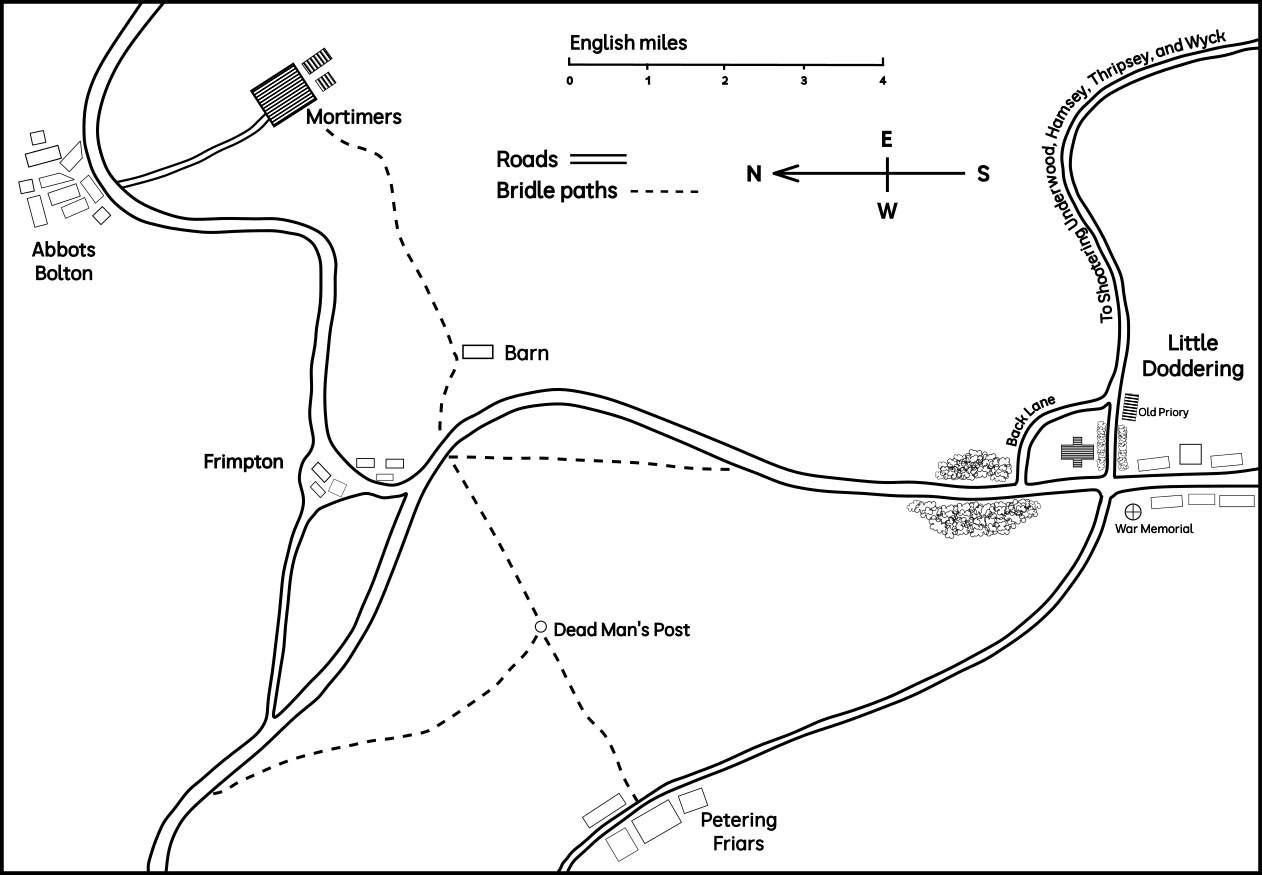
\includegraphics[width=\textwidth]{map}
%\end{center}

The parish church of Little Doddering stands, like so many country churches, at some distance from the houses. The main road from Herriotting, Abbotts Bolton, and Frimpton runs past the west gate of the churchyard—a wide God's acre, crowded with ancient stones. On the south side is a narrow and gloomy lane, heavily overhung with old elm-trees, dividing the church from the still more ancient ruins of Doddering Priory. On the main road, a little beyond the point where Old Priory Lane enters, stands the War Memorial, and from here the road runs straight on into Little Doddering. Round the remaining two sides of the churchyard winds another lane, known to the village simply as the Back Lane. This branches out from the Herriotting road about a hundred yards north of the church, connects with the far end of Priory Lane, and thence proceeds deviously to Shootering Underwood, Hamsey, Thripsey, and Wyck.

»Whatever it was Plunkett thinks he saw,« said Mr~Frobisher-Pym, »it must have come from Shootering. The Back Lane only leads round by some fields and a cottage or two, and it stands to reason anybody coming from Frimpton would have taken the main road, going and coming. The lane is in a very bad state with all this rain. I'm afraid even your detective ability, my dear Wimsey, would not avail to find wheel-marks on this modern tarmac.«

»Hardly,« said Wimsey, »especially in the case of a ghostly chariot which gets along without touching the ground. But your reasoning seems perfectly sound, sir.«

»It was probably a couple of belated wagons going to market,« pursued Mr~Frobisher-Pym, »and the rest of it is superstition and, I am afraid, the local beer. Plunkett couldn't have seen all those details about drivers and hames and so on at this distance. And, if it was making no noise, how did he come to notice it at all, since he'd got past the turn and was walking in the other direction? Depend upon it, he heard the wheels and imagined the rest.«

»Probably,« said Wimsey.

»Of course,« went on his host, »if the wagons really were going about without lights, it ought to be looked into. It is a very dangerous thing, with all these motor vehicles about, and I've had to speak severely about it before now. I fined a man only the other day for the very same thing. Do you care to see the church while we're here?«

Knowing that in country places it is always considered proper to see the church, Lord~Peter expressed his eagerness to do so.

»It's always open nowadays,« said the magistrate, leading the way to the west entrance. »The vicar has an idea that churches should be always open for private prayer. He comes from a town living, of course. Round about here the people are always out on the land, and you can't expect them to come into church in their working clothes and muddy boots. They wouldn't think it respectful, and they've other things to do. Besides, I said to him, consider the opportunity it gives for undesirable conduct. But he's a young man, and he'll have to learn by experience.«

He pushed the door open. A curious, stuffy waft of stale incense, damp, and stoves rushed out at them as they entered—a kind of concentrated extract of Church of England. The two altars, bright with flowers and gilding, and showing as garish splashes among the heavy shadows and oppressive architecture of the little Norman building, sounded the same note of contradiction; it was the warm and human that seemed exotic and unfamiliar; the cold and unwelcoming that seemed native to the place and people.

»This Lady-chapel, as Hancock calls it, in the south aisle, is new, of course,« said Mr~Frobisher-Pym. »It aroused a good deal of opposition, but the Bishop is lenient with the High Church party—too lenient, some people think—but, after all, what does it matter? I'm sure I can say my prayers just as well with two communion-tables as with one. And, I will say for Hancock, he is very good with the young men and the girls. In these days of motor-cycles, it's something to get them interested in religion at all. Those trestles in the chapel are for old Burdock's coffin, I suppose. Ah! Here is the vicar.«

A thin man in a cassock emerged from a door beside the high altar and came down towards them, carrying a tall, oaken candlestick in his hand. He greeted them with a slightly professional smile of welcome. Wimsey diagnosed him promptly as earnest, nervous, and not highly intellectual.

»The candlesticks have only just come,« he observed after the usual introductions had been made. »I was afraid they would not be here in time. However, all is now well.«

He set the candlestick beside the coffin-trestles, and proceeded to decorate its brass spike with a long candle of unbleached wax, which he took from a parcel in a neighbouring pew.

Mr~Frobisher-Pym said nothing. Wimsey felt it incumbent on him to express his interest, and did so.

»It is very gratifying,« said Mr~Hancock, thus encouraged, »to see the people beginning to take a real interest in their church. I have really had very little difficulty in finding watchers for to-night. We are having eight watchers, two by two, from 10 o'clock this evening—till which time I shall be myself on duty—till six in the morning, when I come in to say Mass. The men will carry on till 2 o'clock, then my wife and daughter will relieve them, and Mr~Hubbard and young Rawlinson have kindly consented to take the hours from four till six.«

»What Rawlinson is that?« demanded Mr~Frobisher-Pym.

»Mr~Graham's clerk from Herriotting. It is true he is not a member of the parish, but he was born here, and was good enough to wish to take his turn in watching. He is coming over on his motor-cycle. After all, Mr~Graham has had charge of Burdock's family affairs for very many years, and no doubt they wished to show their respect in some way.«

»Well, I only hope he'll be awake enough to do his work in the morning, after gadding about all night,« said Mr~Frobisher-Pym gruffly. »As for Hubbard, that's his own look-out, though I must say it seems an odd occupation for a publican. Still, if he's pleased, and you're pleased, there's no more to be said about it.«

»You've got a very beautiful old church here, Mr~Hancock,« said Wimsey, seeing that controversy seemed imminent.

»Very beautiful indeed,« said the vicar. »Have you noticed that apse? It is rare for a village church to possess such a perfect Norman apse. Perhaps you would like to come and look at it.« He genuflected as they passed a hanging lamp which burned before a niche. »You see, we are permitted Reservation. The Bishop\longdash« He prattled cheerfully as they wandered up the chancel, digressing from time to time to draw attention to the handsome miserere seats (»Of course, this was the original Priory Church«), and a beautifully carved piscina and aumbry (»It is rare to find them so well preserved«). Wimsey assisted him to carry down the remaining candlesticks from the vestry, and, when these had been put in position, joined Mr~Frobisher-Pym at the door.

\noindent\hfil\rule{0.5\textwidth}{.4pt}\hfil 

»I think you said you were dining with the Lumsdens to-night,« said the magistrate, as they sat smoking after lunch. »How are you going? Will you have the car?«

»I'd rather you'd lend me one of the saddle-horses,« said Wimsey. »I get few opportunities of riding in town.«

»Certainly, my dear boy, certainly. Only I'm afraid you'll have rather a wet ride. Take Polly Flinders; it will do her good to get some exercise. You are quite sure you would prefer it? Have you got your kit with you?«

»Yes—I brought an old pair of bags down with me, and, with this raincoat, I shan't come to any harm. They won't expect me to dress. How far is it to Frimpton, by the way?«

»Nine miles by the main road, and tarmac all the way, I'm afraid, but there's a good wide piece of grass each side. And, of course, you can cut off a mile or so by going across the common. What time will you want to start?«

»Oh, about seven o'clock, I should think. And, I say, sir—will Mrs~Frobisher-Pym think it very rude if I'm rather late back? Old Lumsden and I went through the war together, and if we get yarning over old times we may go on into the small hours. I don't want to feel I'm treating your house like a hotel, but\longdash«

»Of course not, of course not! That's absolutely all right. My wife won't mind in the very least. We want you to enjoy your visit and do exactly what you like. I'll give you the key, and I'll remember not to put the chain up. Perhaps you wouldn't mind doing that yourself when you come in?«

»Rather not. And how about the mare?«

»I'll tell Merridew to look out for you; he sleeps over the stables. I only wish it were going to be a better night for you. I'm afraid the glass is going back. Yes. Dear, dear! It's a bad look-out for to-morrow. By the way, you'll probably pass the funeral procession at the church. It should be along by about then, if the train is punctual.«

The train, presumably, was punctual, for as Lord~Peter cantered up to the west gate of the church he saw a hearse of great funereal pomp drawn up before it, surrounded by a little crowd of people. Two mourning coaches were in attendance; the driver of the second seemed to be having some difficulty with the horses, and Wimsey rightly inferred that this was the pair which had been borrowed from Mr~Mortimer. Restraining Polly Flinders as best he might, he sidled into a respectful position on the edge of the crowd, and watched the coffin taken from the hearse and carried through the gate, where it was met by Mr~Hancock, in full pontificals, attended by a thurifer and two torch-bearers. The effect was a little marred by the rain, which had extinguished the candles, but the village seemed to look upon it as an excellent show nevertheless. A massive man, dressed with great correctness in a black frock coat and tall hat, and accompanied by a woman in handsome mourning and furs, was sympathetically commented on. This was Haviland Burdock of silk-stocking fame, the younger son of the deceased. A vast number of white wreaths were then handed out, and greeted with murmurs of admiration and approval. The choir struck up a hymn, rather raggedly, and the procession filed away into the church. Polly Flinders shook her head vigorously, and Wimsey, taking this as a signal to be gone, replaced his hat and ambled gently away towards Frimpton.

He followed the main road for about four miles, winding up through finely wooded country to the edge of Frimpton Common. Here the road made a wide sweep, skirting the common and curving gently down into Frimpton village. Wimsey hesitated for a moment, considering that it was growing dark and that both the way and the animal he rode were strange to him. There seemed, however, to be a well-defined bridle-path across the common, and eventually he decided to take it. Polly Flinders seemed to know it well enough, and cantered along without hesitation. A ride of about a mile and a half brought them without adventure into the main road again. Here a fork in the road presented itself confusingly; an electric torch, however, and a sign-post solved the problem; after which ten minutes' ride brought the traveller to his goal.

Major Lumsden was a large, cheerful man—none the less cheerful for having lost a leg in the War. He had a large, cheerful wife, a large, cheerful house, and a large, cheerful family. Wimsey soon found himself seated before a fire as large and cheerful as the rest of the establishment, exchanging gossip with his hosts over a whisky-and-soda. He described the Burdock funeral with irreverent gusto, and went on to tell the story of the phantom coach. Major Lumsden laughed.

»It's a quaint part of the country,« he said. »The policeman is just as bad as the rest of them. Do you remember, dear, the time I had to go out and lay a ghost, down at Pogson's farm?«

»I do, indeed,« said his wife emphatically. »The maids had a wonderful time. Trivett—that's our local constable—came rushing in here and fainted in the kitchen, and they all sat round howling and sustaining him with our best brandy, while Dan went down and investigated.«

»Did you find the ghost?«

»Well, not the ghost, exactly, but we found a pair of boots and half a pork-pie in the empty house, so we put it all down to a tramp. Still, I must say odd things do happen about here. There were those fires on the common last year. They were never explained.«

»Gipsies, Dan.«

»Maybe; but nobody ever saw them, and the fires would start in the most unexpected way, sometimes in the pouring rain; and, before you could get near one, it would be out, and only a sodden wet black mark left behind it. And there's another bit of the common that animals don't like—near what they call the Dead Man's Post. My dogs won't go near it. Funny brutes. I've never seen anything there, but even in broad daylight they don't seem to fancy it. The common's not got a good reputation. It used to be a great place for highwaymen.«

»Is the Burdock coach anything to do with highwaymen?«

»No. I fancy it was some rakehelly dead-and-gone Burdock. Belonged to the Hell-fire Club or something. The usual sort of story. All the people round here believe in it, of course. It's rather a good thing. Keeps the servants indoors at night. Well, let's go and have some grub, shall we?«

\noindent\hfil\rule{0.5\textwidth}{.4pt}\hfil 

»Do you remember,« said Major Lumsden, »that damned old mill, and the three elms by the pig-sty?«

»Good Lord, yes! You very obligingly blew them out of the landscape for us, I remember. They made us a damned sight too conspicuous.«

»We rather missed them when they were gone.«

»Thank heaven you didn't miss them when they were there. I'll tell you what you did miss, though.«

»What's that?«

»The old sow.«

»By Jove, yes. Do you remember old Piper fetching her in?«

»I'll say I do. That reminds me. You knew Bunthorne....«

»I'll say good night,« said Mrs~Lumsden, »and leave you people to it.«

»Do you remember,« said Lord~Peter Wimsey, »that awkward moment when Popham went off his rocker?«

»No. I'd been sent back with a batch of prisoners. I heard about it though. I never knew what became of him.«

»I got him sent home. He's married now and living in Lincolnshire.«

»Is he? Well, he couldn't help himself, I suppose. He was only a kid. What's happened to Philpotts?«

»Oh, Philpotts....«

\noindent\hfil\rule{0.5\textwidth}{.4pt}\hfil 

»Where's your glass, old man?«

\noindent\hfil\rule{0.5\textwidth}{.4pt}\hfil 

»Oh, rot, old man. The night is still young....«

\noindent\hfil\rule{0.5\textwidth}{.4pt}\hfil 

»Really? Well, but look here, why not stay the night? My wife will be delighted. I can fix you up in no time.«

»No, thanks most awfully. I must be rolling off home. I said I'd be back; and I'm booked to put the chain on the door.«

»As you like, of course, but it's still raining. Not a good night for a ride on an open horse.«

»I'll bring a saloon next time. We shan't hurt. Rain's good for the complexion—makes the roses grow. Don't wake your man up. I can saddle her myself.«

»My dear man, it's no trouble.«

»No, really, old man.«

»Well, I'll come along and lend you a hand.«

A gust of rain and wind blew in through the hall door as they struggled out into the night. It was past one in the morning and pitch-dark. Major Lumsden again pressed Wimsey to stay.

»No, thanks, really. The old lady's feelings might be hurt. It's not so bad, really—wet, but not cold. Come up, Polly, stand over, old lady.«

He put the saddle on and girthed it, while Lumsden held the lantern. The mare, fed and rested, came delicately dancing out of the warm loose-box, head well stretched forward, and nostrils snuffing at the rain.

»Well, so long, old lad. Come and look us up again. It's been great.«

»Rather! By Jove, yes. Best respects to madame. Is the gate open?«

»Yes.«

»Well, cheerio!«

»Cheerio!«

Polly Flinders, with her nose turned homewards, settled down to make short work of the nine miles of high-road. Once outside the gates, the night seemed lighter, though the rain poured heavily. Somewhere buried behind the thronging clouds there was a moon, which now and again showed as a pale stain on the sky, a paler reflection on the black road. Wimsey, with a mind full of memories and a skin full of whisky, hummed to himself as he rode.

As he passed the fork, he hesitated for a moment. Should he take the path over the common or stick to the road? On consideration, he decided to give the common a miss—not because of its sinister reputation, but because of ruts and rabbit-holes. He shook the reins, bestowed a word of encouragement on his mount, and continued by the road, having the common on his right hand, and, on the left, fields bounded by high hedges, which gave some shelter from the driving rain.

He had topped the rise, and passed the spot where the bridle-path again joined the high-road, when a slight start and stumble drew his attention unpleasantly to Polly Flinders.

»Hold up, mare,« he said disapprovingly.

Polly shook her head, moved forward, tried to pick up her easy pace again. »Hullo!« said Wimsey, alarmed. He pulled her to a standstill.

»Lame in the near fore,« he said, dismounting. »If you've been and gone and strained anything, my girl, four miles from home, father \textit{will} be pleased.« It occurred to him for the first time how curiously lonely the road was. He had not seen a single car. They might have been in the wilds of Africa.

He ran an exploratory hand down the near foreleg. The mare stood quietly enough, without shrinking or wincing. Wimsey was puzzled.

»If these had been the good old days,« he said, »I'd have thought she'd picked up a stone. But what\longdash«

He lifted the mare's foot, and explored it carefully with fingers and pocket-torch. His diagnosis had been right, after all. A steel nut, evidently dropped from a passing car, had wedged itself firmly between the shoe and the frog. He grunted and felt for his knife. Happily, it was one of that excellent old-fashioned kind which includes, besides blades and corkscrews, an ingenious apparatus for removing foreign bodies from horses' feet.

The mare nuzzled him gently as he stooped over his task. It was a little awkward getting to work; he had to wedge the torch under his arm, so as to leave one hand free for the tool and the other to hold the hoof. He was swearing gently at these difficulties when, happening to glance down the road ahead, he fancied he caught the gleam of something moving. It was not easy to see, for at this point the tall trees stood up on both sides of the road, which dipped abruptly from the edge of the common. It was not a car; the light was too faint. A wagon, probably, with a dim lantern. Yet it seemed to move fast. He puzzled for a moment, then bent to work again.

The nut resisted his efforts, and the mare, touched in a tender spot, pulled away, trying to get her foot down. He soothed her with his voice and patted her neck. The torch slipped from his arm. He cursed it impatiently, set down the hoof, and picked up the torch from the edge of the grass, into which it had rolled. As he straightened himself again, he looked along the road and saw.

Up from under the dripping dark of the trees it came, shining with a thin, moony radiance. There was no clatter of hoofs, no rumble of wheels, no ringing of bit or bridle. He saw the white, sleek, shining shoulders with the collar that lay on each, like a faint fiery ring, enclosing nothing. He saw the gleaming reins, their cut ends slipping back and forward unsupported through the ring of the hames. The feet, that never touched earth, ran swiftly—four times four noiseless hoofs, bearing the pale bodies by like smoke. The driver leaned forward, brandishing his whip. He was faceless and headless, but his whole attitude bespoke desperate haste. The coach was barely visible through the driving rain, but Wimsey saw the dimly spinning wheels and a faint whiteness, still and stiff, at the window. It went past at a gallop—headless driver and headless horses and silent coach. Its passing left a stir, a sound that was less a sound than a vibration—and the wind roared suddenly after it, with a great sheet of water blown up out of the south.

»Good God!« said Wimsey. And then: »How many whiskies did we have?«

He turned and looked back along the road, straining his eyes. Then suddenly he remembered the mare, and, without troubling further about the torch, picked up her foot and went to work by touch. The nut gave no more trouble, but dropped out into his hand almost immediately. Polly Flinders sighed gratefully and blew into his ear.

Wimsey led her forward a few steps. She put her feet down firmly and strongly. The nut, removed without delay, had left no tenderness. Wimsey mounted, let her go—then pulled her head round suddenly.

»I'm going to see,« he said resolutely. »Come up, mare! We won't let any headless horses get the better of \textit{us}. Perfectly indecent, goin' about without heads. Get on, old lady. Over the common with you. We'll catch 'em at the cross-roads.«

Without the slightest consideration for his host or his host's property, he put the mare to the bridle-path again, and urged her into a gallop.

At first he thought he could make out a pale, fluttering whiteness, moving away ahead of him on the road. Presently, as high-road and bridle-path diverged, he lost it altogether. But he knew there was no side-road. Bar any accident to his mount, he was bound to catch it before it came to the fork. Polly Flinders, answering easily to the touch of his heel, skimmed over the rough track with the indifference born of familiarity. In less than ten minutes her feet rang out again on the tarmac. He pulled her up, faced round in the direction of Little Doddering, and stared down the road. He could see nothing yet. Either he was well ahead of the coach, or it had already passed at unbelievable speed, or else—

He waited. Nothing. The violent rain had ceased, and the moon was struggling out again. The road appeared completely deserted. He glanced over his shoulder. A small beam of light near the ground moved, turned, flashed green, and red, and white again, and came towards him. Presently he made out that it was a policeman wheeling a bicycle.

»A bad night, sir,« said the man civilly, but with a faint note of enquiry in his voice.

»Rotten,« said Wimsey.

»Just had to mend a puncture, to make it all the pleasanter,« added the policeman.

Wimsey expressed sympathy. »Have you been here long?« he added.

»Best part o' twenty minutes.«

»Did you see anything pass along this way from Little Doddering?«

»Ain't been nothing along while I've been here. What sort of thing did you mean, sir?«

»I thought I saw\longdash« Wimsey hesitated. He did not care about the idea of making a fool of himself. »A carriage with four horses,« he said hesitatingly. »It passed me on this road not a quarter of an hour ago—down at the other end of the common. I—I came back to see. It seemed unusual\longdash« He became aware that his story sounded very lame.

The policeman spoke rather sharply and rapidly.

»There ain't been nothing past here.«

»You're sure?«

»Yes, sir; and, if you don't mind me sayin' so, you'd best be getting home. It's a lonesome bit o' road.«

»Yes, isn't it?« said Wimsey. »Well, good night, sergeant.«

He turned the mare's head back along the Little Doddering road, going very quietly. He saw nothing, heard nothing, and passed nothing. The night was brighter now, and, as he rode back, he verified the entire absence of side-roads. Whatever the thing was which he had seen, it had vanished somewhere along the edge of the common; it had not gone by the main road, nor by any other.

\noindent\hfil\rule{0.5\textwidth}{.4pt}\hfil 

Wimsey came down rather late for breakfast in the morning, to find his hosts in a state of some excitement.

»The most extraordinary thing has happened,« said Mrs~Frobisher-Pym.

»Outrageous!« added her husband. »I warned Hancock—he can't say I didn't warn him. Still, however much one may disapprove of his goings-on, there is no excuse whatever for such abominable conduct. Once let me get hold of the beggars, whoever they are\longdash«

»What's up?« said Wimsey, helping himself to broiled kidneys at the sideboard.

»A most scandalous thing,« said Mrs~Frobisher-Pym. »The vicar came up to Tom at once—I hope we didn't disturb you, by the way, with all the excitement. It appears that when Mr~Hancock got to the church this morning at 6 o'clock to take the early service\longdash«

»No, no, my dear, you've got it wrong. Let \textit{me} tell it. When Joe Grinch—that's the sexton, you know, and he has to get there first to ring the bell—when he arrived, he found the south door wide open and nobody in the chapel, where they should have been, beside the coffin. He was very much perplexed, of course, but he supposed that Hubbard and young Rawlinson had got sick of it and gone off home. So he went on to the vestry to get the vestments and things ready, and to his amazement he heard women's voices, calling out to him from inside. He was so astonished, didn't know where he was, but he went on and unlocked the door\longdash«

»With his own key?« put in Wimsey.

»The key was in the door. As a rule it's kept hanging up on a nail under a curtain near the organ, but it was in the lock—where it ought not to have been. And inside the vestry he found Mrs~Hancock and her daughter, nearly dead with fright and annoyance.«

»Great Scott!«

»Yes, indeed. They had a most extraordinary story to tell. They'd taken over at 2 o'clock from the other pair of watchers, and had knelt down by the coffin in the Lady-chapel, according to plan, to say the proper sort of prayers, whatever they are. They'd been there, to the best of their calculation, about ten minutes, when they heard a noise up by the High Altar, as though somebody was creeping stealthily about. Miss Hancock is a very plucky girl, and she got up and walked up the aisle in the dark, with Mrs~Hancock following on behind because, as she said, she didn't want to be left alone. When they'd got as far as the rood-screen, Miss Hancock called out aloud, 'Who's there?' At that they heard a sort of rustling sound, and a noise like something being knocked over. Miss Hancock most courageously snatched up one of the churchwarden's staffs, which was clipped on to the choir-stalls, and ran forward, thinking, she says, that somebody was trying to steal the ornaments off the altar. There's a very fine fifteenth-century cross\longdash«

»Never mind the cross, Tom. That hasn't been taken, at any rate.«

»No, it hasn't, but she thought it might be. Anyhow, just as she got up to the sanctuary steps, with Mrs~Hancock coming close after her and begging her to be careful, somebody seemed to rush out of the choir-stalls, and caught her by the arms and frog's-marched her—that's her expression—into the vestry. And before she could get breath even to shriek, Mrs~Hancock was pushed in beside her, and the door locked on them.«

»By Jove! You do have exciting times in your village.«

»Well,« said Mr~Frobisher-Pym, »of course they were dreadfully frightened, because they didn't know but what these wretches would come back and murder them, and, in any case, they thought the church was being robbed. But the vestry windows are very narrow and barred, and they couldn't do anything except wait. They tried to listen, but they couldn't hear much. Their only hope was that the four-o'clock watchers might come early and catch the thieves at work. But they waited and they waited, and they heard four strike, and five, and nobody came.«

»What had happened to what's-his-name and Rawlinson then?«

»They couldn't make out, and nor could Grinch. However, they had a good look round the church, and nothing seemed to be taken or disturbed in any way. Just then the vicar came along, and they told him all about it. He was very much shocked, naturally, and his first thought—when he found the ornaments were safe and the poor-box all right—was that some Kensitite people had been stealing the wafers from the what d'you call it.«

»The tabernacle,« suggested Wimsey.

»Yes, that's his name for it. That worried him very much, and he unlocked it and had a look, but the wafers were all there all right, and, as there's only one key, and that was on his own watch-chain, it wasn't a case of anyone substituting unconsecrated wafers for consecrated ones, or any practical joke of that kind. So he sent Mrs~and Miss Hancock home, and had a look round the church outside, and the first thing he saw, lying in the bushes near the south door, was young Rawlinson's motor-cycle.«

»Oho!«

»So his next idea was to hunt for Rawlinson and Hubbard. However, he didn't have to look far. He'd got round the church as far as the furnace-house on the north side, when he heard a terrific hullabaloo going on, and people shouting and thumping on the door. So he called Grinch, and they looked in through the little window, and there, if you please, were Hubbard and young Rawlinson, bawling and going on and using the most shocking language. It seems they were set on in exactly the same way, only before they got inside the church. Rawlinson had been passing the evening with Hubbard, I understand, and they had a bit of a sleep downstairs in the back bar, to avoid disturbing the house early—or so they say, though I dare say if the truth was known they were having drinks; and if that's Hancock's idea of a suitable preparation for going to church and saying prayers, all I can say is, it isn't mine. Anyway, they started off just before four, Hubbard going down on the carrier of Rawlinson's bicycle. They had to get off at the south gate, which was pushed to, and while Rawlinson was wheeling the machine up the path two or three men—they couldn't see exactly—jumped out from the trees. There was a bit of a scuffle, but what with the bicycle, and its being so unexpected, they couldn't put up a very good fight, and the men dropped blankets over their heads, or something. I don't know all the details. At any rate, they were bundled into the furnace-house and left there. They may be there still, for all I know, if they haven't found the key. There should be a spare key, but I don't know what's become of it. They sent up for it this morning, but I haven't seen it about for a long time.«

»It wasn't left in the lock this time, then?«

»No, it wasn't. They've had to send for the locksmith. I'm going down now to see what's to be done about it. Like to come, if you're ready?«

Wimsey said he would. Anything in the nature of a problem always fascinated him.

»You were back pretty late, by the way,« said Mr~Frobisher-Pym jovially, as they left the house. »Yarning over old times, I suppose.«

»We were, indeed,« said Wimsey.

»Hope the old girl carried you all right. Lonely bit of road, isn't it? I don't suppose you saw anybody worse than yourself, as the saying goes?«

»Only a policeman,« said Wimsey untruthfully. He had not yet quite decided about the phantom coach. No doubt Plunkett would be relieved to know that he was not the only person to whom the »warning« had come. But, then, had it really been the phantom coach, or merely a delusion, begotten by whisky upon reminiscence? Wimsey, in the cold light of day, was none too certain.

On arriving at the church, the magistrate and his guest found quite a little crowd collected, conspicuous among whom were the vicar, in cassock and biretta, gesticulating freely, and the local policeman, his tunic buttoned awry and his dignity much impaired by the small fry of the village, who clustered round his legs. He had just finished taking down the statements of the two men who had been released from the stoke-hole. The younger of these, a fresh-faced, impudent-looking fellow of twenty-five or so, was in the act of starting up his motor-cycle. He greeted Mr~Frobisher-Pym pleasantly. »Afraid they've made us look a bit small, sir. You'll excuse me, won't you? I'll have to be getting back to Herriotting. Mr~Graham won't be any too pleased if I'm late for the office. I think some of the bright lads have been having a joke with us.« He grinned as he pushed the throttle-lever over and departed in a smother of unnecessary smoke that made Mr~Frobisher-Pym sneeze. His fellow-victim, a large, fat man, who looked the sporting publican that he was, grinned shamefacedly at the magistrate.

»Well, Hubbard,« said the latter, »I hope you've enjoyed your experience. I must say I'm surprised at a man of your size letting himself be shut up in a coal-hole like a naughty urchin.«

»Yes, sir, I was surprised myself at the time,« retorted the publican, good-humouredly enough. »When that there blanket came down on my head, I was the most surprised man in this here country. I gave 'em a hack or two on the shins, though, to remember me by,« he added, with a reminiscent chuckle.

»How many of them were there?« asked Wimsey.

»Three or four, I should say, sir. But not 'avin' seen 'em, I can only tell from 'earin' 'em talk. There was two laid 'old of me, I'm pretty sure, and young Rawlinson thinks there was only one 'ad 'old of 'im, but 'e was a wonderful strong 'un.«

»We must leave no stone unturned to find out who these people were,« said the vicar excitedly. »Ah, Mr~Frobisher-Pym, come and see what they have done in the church. It is as I thought—an anti-Catholic protest. We must be most thankful that they have done no more than they have.«

He led the way in. Someone had lit two or three hanging lamps in the gloomy little chancel. By their light Wimsey was able to see that the neck of the eagle lectern was decorated with an enormous red-white-and-blue bow, and bore a large placard—obviously pinched from the local newspaper offices—»Vatican Bans Immodest Dress.« In each of the choir-stalls a teddy-bear sat, lumpishly amiable, apparently absorbed in reading the choir-books upside-down, while on the ledge before them copies of the \textit{Pink 'Un} were obstrusively displayed. In the pulpit, a waggish hand had set up a pantomime ass's head, elegantly arrayed in a nightgown, and crowned with a handsome nimbus, cut from gold paper.

»Disgraceful, isn't it?« said the vicar.

»Well, Hancock,« replied Mr~Frobisher-Pym, »I must say I think you have brought it upon yourself—though I quite agree, of course, that this sort of thing cannot possibly be allowed, and the offenders must be discovered and severely punished. But you must see that many of your practices appear to these people to be papistical nonsense at best, and while that is no excuse....«

His reprimanding voice barked on.

»... what I really can only look upon as this sacrilegious business with old Burdock—a man whose life....«

The policeman had by this time shoved away the attendant villagers and was standing beside Lord~Peter at the entrance of the rood-screen.

»Was that you was out on the road this morning, sir? Ah! I thought I reckernised your voice. Did you get home all right, sir? Didn't meet nothing?«

There seemed to be a shade more than idle questioning in the tone of his voice. Wimsey turned quickly.

»No, I met nothing—more. Who is it drives a coach with four white horses about this village of a night, sergeant?«

»Not sergeant, sir—I ain't due for promotion yet awhile. Well, sir, as to white horses, I don't altogether like to say. Mr~Mortimer over at Abbotts Bolton has some nice greys, and he's the biggest horse-breeder about these parts—but, well, there, sir, he wouldn't be driving out in all that rain, sir, would he?«

»It doesn't seem a sensible thing to do, certainly.«

»No, sir. And«—the constable leaned close to Wimsey and spoke into his ear—»and Mr~Mortimer is a man that's got a head on his shoulders—\textit{and, what's more, so have his horses}.«

»Why,« said Wimsey, a little startled by the aptness of this remark, »did you ever know a horse that hadn't?«

»No, sir,« said the policeman, with emphasis, »I never knew no \textit{livin'} horse that hadn't. But that's neether here nor there, as the sayin' goes. But as to this church business, that's just a bit of a lark got up among the boys, that's what that is. They don't mean no harm, you know, sir; they likes to be up to their tricks. It's all very well for the vicar to talk, sir, but this ain't no Kensitites nor anythink of that, as you can see with half an eye. Just a bit of fun, that's all it is.«

»I'd come to the same conclusion myself,« said Wimsey, interested, »but I'd rather like to know what makes you think so.«

»Lord~bless you, sir, ain't it plain as the nose on your face? If it had a-bin these Kensitites, wouldn't they have gone for the crosses and the images and the lights and—that there?» He extended a horny finger in the direction of the tabernacle. «No, sir, these lads what did this ain't laid a finger on the things what you might call sacred images—and they ain't done no harm neether to the communion-table. So I says as it ain't a case of con\textit{trou}versy, but more a bit of fun, like. And they've treated Mr~Burdock's corpse respectful, sir, you see, too. That shows they wasn't meaning anything wrong at heart, don't you see?«

»I agree absolutely,« said Wimsey. »In fact, they've taken particular care not to touch anything that a churchman holds really sacred. How long have you been on this job, officer?«

»Three years, sir, come February.«

»Ever had any idea of going to town or taking up the detective side of the business?«

»Well, sir—I have—but it isn't just ask and have, as you might say.«

Wimsey took a card from his note-case.

»If you ever think seriously about it,« he said, »give this card to Chief Inspector Parker, and have a chat with him. Tell him I think you haven't got opportunities enough down here. He's a great friend of mine, and he'll give you a good chance, I know.«

»I've heard of you, my lord,« said the constable, gratified, »and I'm sure it's very kind of your lordship. Well, I suppose I'd best be getting along now. You leave it to me, Mr~Frobisher-Pym, sir; we'll soon get at the bottom of this here.«

»I hope you do,« said the magistrate. »Meanwhile, Mr~Hancock, I trust you will realise the inadvisability of leaving the church doors open at night. Well, come along, Wimsey; we'll leave them to get the church straight for the funeral. What have you found there?«

»Nothing,« said Wimsey, who had been peering at the floor of the Lady-chapel. »I was afraid you'd got the worm in here, but I see it's only sawdust.« He dusted his fingers as he spoke, and followed Mr~Frobisher-Pym out of the building.

\noindent\hfil\rule{0.5\textwidth}{.4pt}\hfil 

When you are staying in a village, you are expected to take part in the interests and amusements of the community. Accordingly, Lord~Peter duly attended the funeral of Squire Burdock, and beheld the coffin safely committed to the ground, in a drizzle, certainly, but not without the attendance of a large and reverent congregation. After this ceremony, he was formally introduced to Mr~and Mrs~Haviland Burdock, and was able to confirm his previous impression that the lady was well, not to say too well, dressed, as might be expected from one whose wardrobe was based upon silk stockings. She was a handsome woman, in a large, bold style, and the hand that clasped Wimsey's was quite painfully encrusted with diamonds. Haviland was disposed to be friendly—and, indeed, silk manufacturers have no reason to be otherwise to rich men of noble birth. He seemed to be aware of Wimsey's reputation as an antiquarian and book-collector, and extended a hearty invitation to him to come and see the old house.

»My brother Martin is still abroad,« he said, »but I'm sure he would be delighted to have you come and look at the place. I'm told there are some very fine old books in the library. We shall be staying here till Monday—if Mrs~Hancock will be good enough to have us. Suppose you come along to-morrow afternoon.«

Wimsey said he would be delighted.

Mrs~Hancock interposed and said, wouldn't Lord~Peter come to tea at the vicarage first.

Wimsey said it was very good of her.

»Then that's settled,« said Mrs~Burdock. »You and Mr~Pym come to tea, and then we'll all go over the house together. I've hardly seen it myself yet.«

»It's very well worth seeing,« said Mr~Frobisher-Pym. »Fine old place, but takes some money to keep up. Has nothing been seen of the will yet, Mr~Burdock?«

»Nothing whatever,« said Haviland. »It's curious, because Mr~Graham—the solicitor, you know, Lord~Peter—certainly drew one up, just after poor Martin's unfortunate difference with our father. He remembers it perfectly.«

»Can't he remember what's in it?«

»He could, of course, but he doesn't think it etiquette to say. He's one of the crusted old type. Poor Martin always called him an old scoundrel—but then, of course, he never approved of Martin, so Martin was not altogether unprejudiced. Besides, as Mr~Graham says, all that was some years ago, and it's quite possible that the governor destroyed the will later, or made a new one in America.«

»'Poor Martin' doesn't seem to have been popular hereabouts,« said Wimsey to Mr~Frobisher-Pym, as they parted from the Burdocks and turned homewards.

»N-no,« said the magistrate. »Not with Graham, anyway. Personally, I rather liked the lad, though he was a bit harum-scarum. I dare say he's sobered up with time—and marriage. It's odd that they can't find the will. But, if it was made at the time of the rumpus, it's bound to be in Haviland's favour.«

»I think Haviland thinks so,« said Wimsey. »His manner seemed to convey a chastened satisfaction. I expect the discreet Graham made it fairly clear that the advantage was not with the unspeakable Martin.«

The following morning turned out fine, and Wimsey, who was supposed to be enjoying a rest-and-fresh-air cure in Little Doddering, petitioned for a further loan of Polly Flinders. His host consented with pleasure, and only regretted that he could not accompany his guest, being booked to attend a Board of Guardians' meeting in connection with the workhouse.

»But you could go up and get a good blow on the common,« he suggested. »Why not go round by Petering Friars, turn off across the common till you get to Dead Man's Post, and come back by the Frimpton road? It makes a very pleasant round—about nineteen miles. You'll be back in nice time for lunch if you take it easy.«

Wimsey fell in with the plan—the more readily that it exactly coincided with his own inward purpose. He had a reason for wishing to ride over the Frimpton road by daylight.

»You'll be careful about Dead Man's Post,« said Mrs~Frobisher-Pym a little anxiously. »The horses have a way of shying at it. I don't know why. People say, of course\longdash«

»All nonsense,« said her husband. »The villagers dislike the place and that makes the horses nervous. It's remarkable how a rider's feelings communicate themselves to his mount. \textit{I've} never had any trouble at Dead Man's Post.«

It was a quiet and pretty road, even on a November day, that led to Petering Friars. Jogging down the winding Essex lanes in the wintry sunshine, Wimsey felt soothed and happy. A good burst across the common raised his spirits to exhilaration pitch. He had entirely forgotten Dead Man's Post and its uncanny reputation, when a violent start and swerve, so sudden that it nearly unseated him, recalled him to what he was doing. With some difficulty, he controlled Polly Flinders, and brought her to a standstill.

He was at the highest point of the common, following a bridle-path which was bordered on each side by gorse and dead bracken. A little way ahead of him another bridle-path seemed to run into it, and at the junction of the two was something which he had vaguely imagined to be a decayed sign-post. Certainly it was short and thick for a sign-post, and had no arms. It appeared, however, to bear some sort of inscription on the face that was turned towards him.

He soothed the mare, and urged her gently towards the post. She took a few hesitating steps, and plunged sideways, snorting and shivering.

»Queer!« said Wimsey. »If this is my state of mind communicating itself to my mount, I'd better see a doctor. My nerves must be in a rotten state. Come up, old lady! What's the matter with you?«

Polly Flinders, apologetic but determined, refused to budge. He urged her gently with his heel. She sidled away, with ears laid back, and he saw the white of a protesting eye. He slipped from the saddle, and, putting his hand through the bridle, endeavoured to lead her forward. After a little persuasion, the mare followed him, with stretched neck and treading as though on egg-shells. After a dozen hesitating paces, she stopped again, trembling in all her limbs. He put his hand on her neck and found it wet with sweat.

»Damn it all!« said Wimsey. »Look here, I'm jolly well going to read what's on that post. If you won't come, will you stand still?«

He dropped the bridle. The mare stood quietly, with hanging head. He left her and went forward, glancing back from time to time to see that she showed no disposition to bolt. She stood quietly enough, however, only shifting her feet uneasily.

Wimsey walked up to the post. It was a stout pillar of ancient oak, newly painted white. The inscription, too, had been recently blacked in. It read:

\begin{center}\scshape
on this spot\\
george winter\\
was foully murthered\\
in defense of\\
his master's goods\\
by black ralph\\
of herriotting\\
who was afterward\\
hanged in chains\\
on the place of his crime\\
9 november 1674\\
~\\
fear justice
\end{center}

»And very nice, too,« said Wimsey. »Dead Man's Post without a doubt. Polly Flinders seems to share the local feeling about the place. Well, Polly, if them's your sentiments, I won't do violence to them. But may I ask why, if you're so sensitive about a mere post, you should swallow a death-coach and four headless horses with such hardened equanimity?«

The mare took the shoulder of his jacket gently between her lips and mumbled at it.

»Just so,« said Wimsey. »I perfectly understand. You would if you could, but you really can't. But those horses, Polly—did they bring with them no brimstone blast from the nethermost pit? Can it be that they really exuded nothing but an honest and familiar smell of stables?«

He mounted, and, turning Polly's head to the right, guided her in a circle, so as to give Dead Man's Post a wide berth before striking the path again.

»The supernatural explanation is, I think, excluded. Not on \textit{a priori} grounds, which would be unsound, but on the evidence of Polly's senses. There remain the alternatives of whisky and jiggery-pokery. Further investigation seems called for.«

He continued to muse as the mare moved quietly forward.

»Supposing I wanted, for some reason, to scare the neighbourhood with the apparition of a coach and headless horses, I should choose a dark, rainy night. Good! It was that kind of night. Now, if I took black horses and painted their bodies white—poor devils! what a state they'd be in. No. How do they do these Maskelyne-and-Devant stunts where they cut off people's heads? White horses, of course—and black felt clothing over their heads. Right! And luminous paint on the harness, with a touch here and there on their bodies, to make good contrast and ensure that the whole show wasn't invisible. No difficulty about that. But they must go silently. Well, why not? Four stout black cloth bags filled with bran, drawn well up and tied round the fetlocks would make any horse go quietly enough, especially if there was a bit of a wind going. Rags round the bridle-rings to prevent clinking, and round the ends of the traces to keep 'em from squeaking. Give 'em a coachman in a white coat and a black mask, hitch 'em to a rubber-tyred fly, picked out with phosphorus and well-oiled at the joints—and I swear I'd make something quite ghostly enough to startle a rather well-irrigated gentleman on a lonely road at half-past two in the morning.«

He was pleased with this thought, and tapped his boot cheerfully with his whip.

»But damn it all! They never passed me again. Where did they go to? A coach-and-horses can't vanish into thin air, you know. There must be a side-road after all—or else, Polly Flinders, you've been pulling my leg all the time.«

The bridle-path eventually debouched upon the highway at the now familiar fork where Wimsey had met the policeman. As he slowly ambled homewards, his lordship scanned the left-hand hedgerow, looking for the lane which surely must exist. But nothing rewarded his search. Enclosed fields with padlocked gates presented the only breaks in the hedge, till he again found himself looking down the avenue of trees up which the death-coach had come galloping two nights before.

»Damn!« said Wimsey.

It occurred to him for the first time that the coach might perhaps have turned round and gone back through Little Doddering. Certainly it had been seen by Little Doddering Church on Wednesday. But on that occasion, also, it had galloped off in the direction of Frimpton. In fact, thinking it over, Wimsey concluded that it had approached from Frimpton, gone round the church—widdershins, naturally—by the Back Lane, and returned by the high-road whence it came. But in that case—

»Turn again, Whittington,« said Wimsey, and Polly Flinders rotated obediently in the road. »Through one of those fields it went, or I'm a Dutchman.«

He pulled Polly into a slow walk, and passed along the strip of grass at the right-hand side, staring at the ground as though he were an Aberdonian who had lost a sixpence.

The first gate led into a ploughed field, harrowed smooth and sown with autumn wheat. It was clear that no wheeled thing had been across it for many weeks. The second gate looked more promising. It gave upon fallow ground, and the entrance was seamed with innumerable wheel-ruts. On further examination, however, it was clear that this was the one and only gate. It seemed unlikely that the mysterious coach should have been taken into a field from which there was no way out. Wimsey decided to seek farther.

The third gate was in bad repair. It sagged heavily from its hinges; the hasp was gone, and gate and post had been secured with elaborate twists of wire. Wimsey dismounted and examined these, convincing himself that their rusty surface had not been recently disturbed.

There remained only two more gates before he came to the cross-roads. One led into plough again, where the dark ridge-and-furrow showed no sign of disturbance, but at sight of the last gate Wimsey's heart gave a leap.

There was plough-land here also, but round the edge of the field ran a wide, beaten path, rutted and water-logged. The gate was not locked, but opened simply with a spring catch. Wimsey examined the approach. Among the wide ruts made by farm-wagons was the track of four narrow wheels—the unmistakable prints of rubber tyres. He pushed the gate open and passed through.

The path skirted two sides of the plough; then came another gate and another field, containing a long barrow of mangold wurzels and a couple of barns. At the sound of Polly's hoofs, a man emerged from the nearest barn, with a paint-brush in his hand, and stood watching Wimsey's approach.

»'Morning!« said the latter genially.

»'Morning, sir.«

»Fine day after the rain.«

»Yes, it is, sir.«

»I hope I'm not trespassing?«

»Where was you wanting to go, sir?«

»I thought, as a matter of fact—hullo!«

»Anything wrong, sir?«

Wimsey shifted in the saddle.

»I fancy this girth's slipped a bit. It's a new one.« (This was a fact.) »Better have a look.«

The man advanced to investigate, but Wimsey had dismounted and was tugging at the strap, with his head under the mare's belly.

»Yes, it wants taking up a trifle. Oh! Thanks most awfully. Is this a short cut to Abbotts Bolton, by the way?«

»Not to the village, sir, though you can get through this way. It comes out by Mr~Mortimer's stables.«

»Ah, yes. This his land?«

»No, sir, it's Mr~Topham's land, but Mr~Mortimer rents this field and the next for fodder.«

»Oh, yes.« Wimsey peered across the hedge. »Lucerne, I suppose. Or clover.«

»Clover, sir. And the mangolds is for the cattle.«

»Oh—Mr~Mortimer keeps cattle as well as horses?«

»Yes, sir.«

»Very jolly. Have a gasper?« Wimsey had sidled across to the barn in his interest, and was gazing absently into its dark interior. It contained a number of farm implements and a black fly of antique construction, which seemed to be undergoing renovation with black varnish. Wimsey pulled some vestas from his pocket. The box was apparently damp, for, after one or two vain attempts he abandoned it, and struck a match on the wall of the barn. The flame, lighting up the ancient fly, showed it to be incongruously fitted with rubber tyres.

»Very fine stud, Mr~Mortimer's, I understand,« said Wimsey carelessly.

»Yes, sir, very fine indeed.«

»I suppose he hasn't any greys, by any chance. My mother—queenly woman, Victorian ideas, and all that—is rather keen on greys. Sports a carriage and pay-ah, don't you know.«

»Yes, sir? Well, Mr~Mortimer would be able to suit the lady, I think, sir. He has several greys.«

»No? has he though? I must really go over and see him. Is it far?«

»Matter of five or six mile by the fields, sir.«

Wimsey looked at his watch.

»Oh, dear! I'm really afraid it's too far for this morning. I absolutely promised to get back to lunch. I must come over another day. Thanks \textit{so} much. Is that girth right now? Oh, really, I'm immensely obliged. Get yourself a drink, won't you—and tell Mr~Mortimer not to sell his greys till I've seen them. Well, \textit{good} morning, and many thanks.«

He set Polly Flinders on the homeward path and trotted gently away. Not till he was out of sight of the barn did he pull up and, stooping from the saddle, thoughtfully examine his boots. They were liberally plastered with bran.

»I must have picked it up in the barn,« said Wimsey. »Curious, if true. Why should Mr~Mortimer be lashing the stuffing out of his greys in an old fly at dead of night—and with muffled hoofs and no heads to boot? It's not a kind thing to do. It frightened Plunkett very much. It made me think I was drunk—a thought I hate to think. Ought I to tell the police? Are Mr~Mortimer's jokes any business of mine? What do \textit{you} think, Polly?«

The mare, hearing her name, energetically shook her head.

»You think not? Perhaps you are right. Let us say that Mr~Mortimer did it for a wager. Who am I to interfere with his amusements? All the same,« added his lordship, »I'm glad to know it wasn't Lumsden's whisky.«

\noindent\hfil\rule{0.5\textwidth}{.4pt}\hfil 

»This is the library,« said Haviland, ushering in his guests. »A fine room—and a fine collection of books, I'm told, though literature isn't much in my line. It wasn't much in the governor's line, either, I'm afraid. The place wants doing up, as you see. I don't know whether Martin will take it in hand. It's a job that'll cost money, of course.«

Wimsey shivered a little as he gazed round—more from sympathy than from cold, though a white November fog lay curled against the tall windows and filtered damply through the frames.

A long, mouldering room, in the frigid neo-classical style, the library was melancholy enough in the sunless grey afternoon, even without the signs of neglect which wrung the book-collector's heart. The walls, panelled to half their height with book-cases, ran up in plaster to the moulded ceiling. Damp had blotched them into grotesque shapes, and here and there were ugly cracks and squamous patches, from which the plaster had fallen in yellowish flakes. A wet chill seemed to ooze from the books, from the calf bindings peeling and perishing, from the stains of greenish mildew which spread horridly from volume to volume. The curious musty odour of decayed leather and damp paper added to the general cheerlessness of the atmosphere.

»Oh, dear, dear!« said Wimsey, peering dismally into this sepulchre of forgotten learning. With his shoulders hunched like the neck-feathers of a chilly bird, with his long nose and half-shut eyes, he resembled a dilapidated heron, brooding over the stagnation of a wintry pool.

»What a freezing-cold place!« exclaimed Mrs~Hancock. »You really ought to scold Mrs~Lovall, Mr~Burdock. When she was put in here as caretaker, I said to my husband—didn't I, Philip?—that your father had chosen the laziest woman in Little Doddering. She ought to have kept up big fires here, \textit{at least} twice a week! It's really shameful, the way she has let things go.«

»Yes, isn't it?« agreed Haviland.

Wimsey said nothing. He was nosing along the shelves, every now and then taking a volume down and glancing at it.

»It was always rather a depressing room,« went on Haviland. »I remember, when I was a kid, it used to overawe me rather. Martin and I used to browse about among the books, you know, but I think we were always afraid that something or somebody would stalk out upon us from the dark corners. What's that you've got there, Lord~Peter? Oh, \textit{Foxe's Book of Martyrs}. Dear me! How those pictures did terrify me in the old days! And there was a \textit{Pilgrim's Progress}, with a most alarming picture of Apollyon straddling over the whole breadth of the way, which gave me many nightmares. Let me see. It used to live over in this bay, I think. Yes, here it is. How it does bring it all back, to be sure! Is it valuable, by the way?«

»No, not really. But this first edition of Burton is worth money; badly spotted, though—you'd better send it to be cleaned. And this is an extremely fine Boccaccio; take care of it.«

»John Boccace—\textit{The Dance of Machabree}. It's a good title, anyhow. Is that the same Boccaccio that wrote the naughty stories?«

»Yes,« said Wimsey, a little shortly. He resented this attitude towards Boccaccio.

»Never read them,« said Haviland, with a wink at his wife, »but I've seen 'em in the windows of those surgical shops—so I suppose they're naughty, eh? The vicar's looking shocked.«

»Oh, not at all,« said Mr~Hancock, with a conscientious assumption of broad-mindedness. »Et ego in Arcadia—that is to say, one doesn't enter the Church without undergoing a classical education, and making the acquaintance of much more worldly authors even than Boccaccio. Those wood-cuts are very fine, to my uninstructed eye.«

»Very fine indeed,« said Wimsey.

»There's another old book I remember, with jolly pictures,« said Haviland. »A chronicle of some sort—what's 'is name—place in Germany—\textit{you} know—where that hangman came from. They published his diary the other day. I read it, but it wasn't really exciting; not half as gruesome as old Harrison Ainsworth. What's the name of the place?«

»Nüremberg?« suggested Wimsey.

»That's it, of course—the \textit{Nüremberg \textit{Chronicle}}. I wonder if that's still in its old place. It was over here by the window, if I remember rightly.«

He led the way to the end of one of the bays, which ran up close against a window. Here the damp seemed to have done its worst. A pane of glass was broken, and rain had blown in.

»Now where has it gone to? A big book, it was, with a stamped leather binding. I'd like to see the old \textit{\textit{Chronicle}} again. I haven't set eyes on it for donkey's years.«

His glance roamed vaguely over the shelves. Wimsey, with the book-lover's instinct, was the first to spot the \textit{\textit{Chronicle}}, wedged at the extreme end of the shelf, against the outer wall. He hitched his finger into the top edge of the spine, but finding that the rotting leather was ready to crumble at a touch, he dislodged a neighbouring book and drew the \textit{\textit{Chronicle}} gently out, using his whole hand.

»Here he is—in pretty bad condition, I'm afraid. Hullo!«

As he drew the book away from the wall, a piece of folded parchment came away with it and fell at his feet. He stooped and picked it up.

»I say, Burdock—isn't this what you've been looking for?«

Haviland Burdock, who had been rooting about on one of the lower shelves, straightened himself quickly, his face red from stooping.

»By Jove!« he said, turning first redder and then pale with excitement. »Look at this, Winnie. It's the governor's will. What an extraordinary thing! Whoever would have thought of looking for it here, of all places?«

»Is it really the will?« cried Mrs~Hancock.

»No doubt about it, I should say,« observed Wimsey coolly. »Last Will and Testament of Simon Burdock.« He stood, turning the grimy document over and over in his hands, looking from the endorsement to the plain side of the folded parchment.

»Well, well!« said Mr~Hancock. »How strange! It seems almost providential that you should have taken that book down.«

»What does the will say?« demanded Mrs~Burdock, in some excitement.

»I beg your pardon,« said Wimsey, handing it over to her. »Yes, as you say, Mr~Hancock, it does almost seem as if I was meant to find it.« He glanced down again at the \textit{Chronicle}, mournfully tracing with his finger the outline of a damp stain which had rotted the cover and spread to the inner pages, almost obliterating the colophon.

Haviland Burdock meanwhile had spread the will out on the nearest table. His wife leaned over his shoulder. The Hancocks, barely controlling their curiosity, stood near, awaiting the result. Wimsey, with an elaborate pretence of non-interference in this family matter, examined the wall against which the \textit{Chronicle} had stood, feeling its moist surface and examining the damp-stains. They had assumed the appearance of a grinning face. He compared them with the corresponding mark on the book, and shook his head desolately over the damage.

Mr~Frobisher-Pym, who had wandered away some time before and was absorbed in an ancient book of Farriery, now approached, and enquired what the excitement was about.

»Listen to this!« cried Haviland. His voice was quiet, but a suppressed triumph throbbed in it and glittered from his eyes.

»»I bequeath everything of which I die possessed«—there's a lot of enumeration of properties here, which doesn't matter—»to my eldest son, Martin«\longdash«

Mr~Frobisher-Pym whistled.

»Listen! »To my eldest son Martin, for so long as my body shall remain above ground. But so soon as I am buried, I direct that the whole of this property shall revert to my younger son Haviland absolutely«\longdash«

»Good God!« said Mr~Frobisher-Pym.

»There's a lot more,« said Haviland, »but that's the gist of it.«

»Let me see,« said the magistrate.

He took the will from Haviland, and read it through with a frowning face.

»That's right,« he said. »No possible doubt about it. Martin has had his property and lost it again. How very curious. Up till yesterday everything belonged to him, though nobody knew it. Now it is all yours, Burdock. This certainly is the strangest will I ever saw. Just fancy that. Martin the heir, up to the time of the funeral. And now—well, Burdock, I must congratulate you.«

»Thank you,« said Haviland. »It is very unexpected.« He laughed unsteadily.

»But what a queer idea!« cried Mrs~Burdock. »Suppose Martin had been at home. It almost seems a mercy that he wasn't, doesn't it? I mean, it would all have been so awkward. What would have happened if he had tried to stop the funeral, for instance?«

»Yes,« said Mrs~Hancock. »Could he have done anything? Who decides about funerals?«

»The executors, as a rule,« said Mr~Frobisher-Pym.

»Who are the executors in this case?« enquired Wimsey.

»I don't know. Let me see.« Mr~Frobisher-Pym examined the document again. »Ah, yes! Here we are. 'I appoint my two sons, Martin and Haviland, joint executors of this my will.' What an extraordinary arrangement.«

»I call it a wicked, un-Christian arrangement,« cried Mrs~Hancock. »It might have caused dreadful mischief if the will hadn't been—quite providentially—lost!«

»Hush, my dear!« said her husband.

»I'm afraid,« said Haviland grimly, »that that was my father's idea. It's no use my pretending he wasn't spiteful; he was, and I believe he hated both Martin and me like poison.«

»Don't say that,« pleaded the vicar.

»I do say it. He made our lives a burden to us, and he obviously wanted to go on making them a burden after he was dead. If he'd seen us cutting each other's throats, he'd only have been too pleased. Come, vicar, it's no use pretending. He hated our mother and was jealous of us. Everybody knows that. It probably pleased his unpleasant sense of humour to think of us squabbling over his body. Fortunately, he over-reached himself when he hid the will here. He's buried now, and the problem settles itself.«

»Are you quite sure of that?« said Wimsey.

»Why, of course,« said the magistrate. »The property goes to Mr~Haviland Burdock as soon as his father's body is underground. Well, his father was buried yesterday.«

»But are you sure of \textit{that}?« repeated Wimsey. He looked from one to the other quizzically, his long lips curling into something like a grin.

»Sure of that?« exclaimed the vicar. »My dear Lord~Peter, you were present at the funeral. You saw him buried yourself.«

»I saw his coffin buried,« said Wimsey mildly. »That the body was in it is merely an unverified inference.«

»I think,« said Mr~Frobisher-Pym, »this is rather an unseemly kind of jest. There is no reason to imagine that the body was not in the coffin.«

»I saw it in the coffin,« said Haviland, »and so did my wife.«

»And so did I,« said the vicar. »I was present when it was transferred from the temporary shell in which it crossed over from the States to a permanent lead-and-oak coffin provided by Joliffe. And, if further witnesses are necessary, you can easily get Joliffe himself and his men, who put the body in and screwed it down.«

»Just so,« said Wimsey. »I'm not denying that the body was in the coffin when the coffin was placed in the chapel. I only doubt whether it was there when it was put in the ground.«

»That is a most unheard-of suggestion to make, Lord~Peter,« said Mr~Frobisher-Pym, with severity. »May I ask if you have anything to go upon? And, if the body is not in the grave, perhaps you wouldn't mind telling us where you imagine it to be?«

»Not at all,« said Wimsey. He perched himself on the edge of the table and sat, swinging his legs and looking down at his own hands, as he ticked his points off on his fingers.

»I think,« he said, »that this story begins with young Rawlinson. He is a clerk in the office of Mr~Graham, who drew up this will, and I fancy he knows something about its conditions. So, of course, does Mr~Graham, but I don't somehow suspect \textit{him} of being mixed up in this. From what I can hear, he is not a man to take sides—or not Mr~Martin's side, at any rate.

When the news of Mr~Burdock's death was cabled over from the States, I think young Rawlinson remembered the terms of the will, and considered that Mr~Martin—being abroad and all that—would be rather at a disadvantage. Rawlinson must be rather attached to your brother, by the way\longdash«

»Martin always had a way of picking up good-for-nothing youths and wasting his time with them,« agreed Haviland sulkily.

The vicar seemed to feel that this statement needed some amendment, and murmured that he had always heard how good Martin was with the village lads.

»Quite so,« said Wimsey. »Well, I think young Rawlinson wanted to give Martin an equal chance of securing the legacy, don't you see. He didn't like to say anything about the will—which might or might not turn up—and possibly he thought that even if it did turn up there might be difficulties. Well, anyway, he decided that the best thing to do was to steal the body and keep it above-ground till Martin came home to see to things himself.«

»This is an extraordinary accusation,« began Mr~Frobisher-Pym.

»I dare say I'm mistaken,« said Wimsey, »but it's just my idea. It makes a damn good story, anyhow—you see! Well, then, young Rawlinson saw that this was too big a job to carry out alone, so he looked round for somebody to help him. And he pitched on Mr~Mortimer.«

»Mortimer?«

»I don't know Mr~Mortimer personally, but he seems to be a sportin' sort of customer from what I can hear, with certain facilities which everybody hasn't got. Young Rawlinson and Mortimer put their heads together and worked out a plan of action. Of course, Mr~Hancock, you helped them enormously with this lying-in-state idea of yours. Without that, I don't know if they could have worked it.«

Mr~Hancock made an embarrassed clucking sound.

»The idea was this. Mortimer was to provide an antique fly and four white horses, made up with luminous paint and black cloth to represent the Burdock death-coach. The advantage of that idea was that nobody would feel inclined to inspect the turn-out too closely if they saw it hangin' round the churchyard at unearthly hours. Meanwhile, young Rawlinson had to get himself accepted as a watcher for the chapel, and to find a sporting companion to watch with him and take a hand in the game. He fixed things up with the publican-fellow, and spun a tale for Mr~Hancock, so as to get the vigil from four to six. Didn't it strike you as odd, Mr~Hancock, that he should be so keen to come all the way from Herriotting?«

»I am accustomed to find keenness in my congregation,« said Mr~Hancock stiffly.

»Yes, but Rawlinson didn't belong to your congregation. Anyway it was all worked out, and there was a dress-rehearsal on the Wednesday night, which frightened your man Plunkett into fits, sir.«

»If I thought this was true\longdash« said Mr~Frobisher-Pym.

»On Thursday night,« pursued Wimsey, »the conspirators were ready, hidden in the chancel at two in the morning. They waited till Mrs~and Miss Hancock had taken their places, and then made a row to attract their attention. When the ladies courageously advanced to find out what was up, they popped out and bundled 'em into the vestry.«

»Good gracious!« said Mrs~Hancock.

»That was when the death-coach affair was timed to drive up to the south door. It came round the Back Lane, I fancy, though I can't be sure. Then Mortimer and the other two took the embalmed body out of the coffin and filled its place up with bags of sawdust. I know it was sawdust, because I found the remains of it on the Lady-chapel floor in the morning. They put the body in the fly, and Mortimer drove off with it. They passed me on the Herriotting Road at half-past two, so they can't have wasted much time over the job. Mortimer may have been alone, or possibly he had someone with him to see to the body while he himself did the headless coachman business in a black mask. I'm not certain about that. They drove through the last gate before you come to the fork at Frimpton, and went across the fields to Mortimer's barn. They left the fly there—I know that, because I saw it, and I saw the bran they used to muffle the horses' hoofs, too. I expect they took it on from there in a car, and fetched the horses up next day—but that's a detail. I don't know, either, where they took the body to, but I expect, if you went and asked Mortimer about it, he would be able to assure you that it was still above ground.«

Wimsey paused. Mr~Frobisher-Pym and the Hancocks were looking only puzzled and angry, but Haviland's face was green. Mrs~Haviland showed a red, painted spot on each cheek, and her mouth was haggard. Wimsey picked up the \textit{Nüremberg Chronicle} and caressed its covers thoughtfully as he went on.

»Meanwhile, of course, young Rawlinson and his companion were doing the camouflage in the church, to give the idea of a Protestant outrage. Having fixed everything up neat and pretty, all they had to do was to lock themselves up in the furnace-house and chuck the key through the window. You'll probably find it there, Mr~Hancock, if you care to look. Didn't you think that story of an assault by two or three men was a bit thin? Hubbard is a hefty great fellow, and Rawlinson's a sturdy lad—and yet, on their own showing, they were bundled into a coal-hole like helpless infants, without a scratch on either of 'em. Look for the men in buckram, my dear sir, look for the men in buckram!«

»Look here, Wimsey, are you sure you're not romancing?« said Mr~Frobisher-Pym. »One would need some very clear proof before\longdash«

»Certainly,« said Wimsey. »Get a Home Office order. Open the grave. You'll soon see whether it's true or whether it's just my diseased imagination.«

»I think this whole conversation is disgusting,« cried Mrs~Burdock. »Don't listen to it, Haviland. Anything more heartless on the day after father's funeral than sitting here and inventing such a revolting story I simply can't imagine. It is not worth paying a moment's attention to. You will certainly not permit your father's body to be disturbed. It's horrible. It's a desecration.«

»It is very unpleasant indeed,« said Mr~Frobisher-Pym gravely, »but if Lord~Peter is seriously putting forward this astonishing theory, which I can scarcely credit\longdash«

Wimsey shrugged his shoulders.

»—then I feel bound to remind you, Mr~Burdock, that your brother, when he returns, may insist on having the matter investigated.«

»But he can't, can he?« said Mrs~Burdock.

»Of course he can, Winnie,« snapped her husband savagely. »He's an executor. He has as much right to have the governor dug up as I have to forbid it. Don't be a fool.«

»If Martin had any decency, he would forbid it, too,« said Mrs~Burdock.

»Oh, well!« said Mrs~Hancock, »shocking as it may seem, there's the money to be considered. Mr~Martin might think it a duty to his wife, and his family, if he should ever have any\longdash«

»The whole thing is preposterous,« said Haviland decidedly. »I don't believe a word of it. If I did, naturally I should be the first person to take action in the matter—not only in justice to Martin, but on my own account. But if you ask me to believe that a responsible man like Mortimer would purloin a corpse and desecrate a church—the thing only has to be put into plain words to show how absurd and unthinkable it is. I suppose Lord~Peter Wimsey, who consorts, as I understand, with criminals and police officers, finds the idea conceivable. I can only say that I do not. I am sorry that his mind should have become so blunted to all decent feeling. That's all. Good afternoon.«

Mr~Frobisher-Pym jumped up.

»Come, come, Burdock, don't take that attitude. I am sure Lord~Peter intended no discourtesy. I must say I think he's all wrong, but, 'pon my soul, things have been so disturbed in the village these last few days, I'm not surprised anybody should think there was something behind it. Now, let's forget about it—and hadn't we better be moving out of this terribly cold room? It's nearly dinner-time. Bless me, what will Agatha think of us?«

Wimsey held out his hand to Burdock, who took it reluctantly.

»I'm sorry,« said Wimsey. »I suffer from hypertrophy of the imagination, y'know. Over-stimulation of the thyroid probably. Don't mind me. I apologise, and all that.«

»I don't think, Lord~Peter,« said Mrs~Burdock acidly, »you ought to exercise your imagination at the expense of good taste.«

Wimsey followed her from the room in some confusion. Indeed, he was so disturbed that he carried away the \textit{Nüremberg Chronicle} beneath his arm, which was an odd thing for him to do under the circumstances.

\noindent\hfil\rule{0.5\textwidth}{.4pt}\hfil 

»I am gravely distressed,« said Mr~Hancock.

He had come over, after Sunday evening service, to call upon the Frobisher-Pyms. He sat upright on his chair, his thin face flushed with anxiety.

»I could never have believed such a thing of Hubbard. It has been a grievous shock to me. It is not only the great wickedness of stealing a dead body from the very precincts of the church, though that is grave enough. It is the sad hypocrisy of his behaviour—the mockery of sacred things—the making use of the holy services of his religion to further worldly ends. He actually attended the funeral, Mr~Frobisher-Pym, and exhibited every sign of grief and respect. Even now he hardly seems to realise the sinfulness of his conduct. I feel it very much, as a priest and as a pastor—very much indeed.«

»Oh, well, Hancock,« said Mr~Frobisher-Pym, »you must make allowances, you know. Hubbard's not a bad fellow, but you can't expect refinement of feeling from a man of his class. The point is, what are we to do about it? Mr~Burdock must be told, of course. It's a most awkward situation. Dear me! Hubbard confessed the whole conspiracy, you say? How did he come to do that?«

»I taxed him with it,« said the parson. »When I came to think over Lord~Peter Wimsey's remarks, I was troubled in my mind. It seemed to me—I cannot say why—that there might be some truth in the story, wild as it appeared. I was so worried about it that I swept the floor of the Lady-chapel myself last night, and I found quite a quantity of sawdust among the sweepings. That led me to search for the key of the furnace-house, and I discovered it in some bushes at a little distance—in fact, within a stone's throw—of the furnace-house window. I sought guidance in prayer—and from my wife, whose judgment I greatly respect—and I made up my mind to speak to Hubbard after Mass. It was a great relief to me that he did not present himself at Early Celebration. Feeling as I did, I should have had scruples.«

»Just so, just so,« said the magistrate, a little impatiently. »Well, you taxed him with it, and he confessed?«

»He did. I am sorry to say he showed no remorse at all. He even laughed. It was a most painful interview.«

»I am sure it must have been,« said Mrs~Frobisher-Pym sympathetically.

»We must go and see Mr~Burdock,« said the magistrate, rising. »Whatever old Burdock may or may not have intended by that iniquitous will of his, it's quite evident that Hubbard and Mortimer and Rawlinson were entirely in the wrong. Upon my word, I've no idea whether it's an indictable offence to steal a body. I must look it up. But I should say it was. If there is any property in a corpse, it must belong to the family or the executors. And in any case, it's sacrilege, to say nothing of the scandal in the parish. I must say, Hancock, it won't do us any good in the eyes of the Nonconformists. However, no doubt you realise that. Well, it's an unpleasant job, and the sooner we tackle it the better. I'll run over to the vicarage with you and help you to break it to the Burdocks. How about you, Wimsey? You were right, after all, and I think Burdock owes you an apology.«

»Oh, I'll keep out of it,« said Wimsey. »I shan't be exactly \textit{persona grata}, don't you know. It's going to mean a deuce of a big financial loss to the Haviland Burdocks.«

»So it is. Most unpleasant. Well, perhaps you're right. Come along, vicar.«

Wimsey and his hostess sat discussing the matter by the fire for half an hour or so, when Mr~Frobisher-Pym suddenly put his head in and said:

»I say, Wimsey—we're all going over to Mortimer's. I wish you'd come and drive the car. Merridew always has the day off on Sunday, and I don't care about driving at night, particularly in this fog.«

»Right you are,« said Wimsey. He ran upstairs, and came down in a few moments wearing a heavy leather flying-coat, and with a parcel under his arm. He greeted the Burdocks briefly, climbed into the driving-seat, and was soon steering cautiously through the mist along the Herriotting Road.

He smiled a little grimly to himself as they came up under the trees to the spot where the phantom coach had passed him. As they passed the gate through which the ingenious apparition had vanished, he indulged himself by pointing it out, and was rewarded by hearing a snarl from Haviland. At the well-remembered fork, he took the right-hand turning into Frimpton and drove steadily for six miles or so, till a warning shout from Mr~Frobisher-Pym summoned him to look out for the turning up to Mortimer's.

Mr~Mortimer's house, with its extensive stabling and farm buildings, stood about two miles back from the main road. In the darkness Wimsey could see little of it; but he noticed that the ground-floor windows were all lit up, and, when the door opened to the magistrate's imperative ring, a loud burst of laughter from the interior gave evidence that Mr~Mortimer was not taking his misdoings too seriously.

»Is Mr~Mortimer at home?« demanded Mr~Frobisher-Pym, in the tone of a man not to be trifled with.

»Yes, sir. Will you come in, please?«

They stepped into a large, old-fashioned hall, brilliantly lit, and made cosy with a heavy oak screen across the door. As Wimsey advanced, blinking, from the darkness, he saw a large, thick-set man, with a ruddy face, advancing with hand outstretched in welcome.

»Frobisher-Pym! By Jove! how decent of you to come over! We've got some old friends of yours here. Oh!« (in a slightly altered tone) »Burdock! Well, well\longdash«

»Damn you!« said Haviland Burdock, thrusting furiously past the magistrate, who was trying to hold him back. »Damn you, you swine! Chuck this bloody farce. What have you done with the body?«

»The body, eh?« said Mr~Mortimer, retreating in some confusion.

»Yes, curse you! Your friend Hubbard's split. It's no good denying it. What the devil do you mean by it? You've got the body here somewhere. Where is it? Hand it over!«

He strode threateningly round the screen into the lamplight. A tall, thin man rose up unexpectedly from the depths of an arm-chair and confronted him.

»Hold hard, old man!«

»Good God!« said Haviland, stepping heavily back on Wimsey's toes. »Martin!«

»Sure,« said the other. »Here I am. Come back like a bad half-penny. How are you?«

»So \textit{you're} at the bottom of this!« stormed Haviland. »I might have known it. You damned, dirty hound! I suppose you think it's decent to drag your father out of his coffin and tote him about the country like a circus. It's degrading. It's disgusting. It's abominable. You must be perfectly dead to all decent feeling. You don't deny it, I suppose?«

»I say, Burdock!« expostulated Mortimer.

»Shut up, curse you!« said Haviland. »I'll deal with you in a minute. Now, look here, Martin, I'm not going to stand any more of this disgraceful behaviour. You'll give up that body, and\longdash«

»Just a moment, just a moment,« said Martin. He stood, smiling a little, his hands thrust into the pockets of his dinner-jacket. »This \textit{éclaircissement} seems to be rather public. Who are all these people? Oh, it's the vicar, I see. I'm afraid we owe you a little explanation, vicar. And, er\longdash«

»This is Lord~Peter Wimsey,« put in Mr~Frobisher-Pym, »who discovered your—I'm afraid, Burdock, I must agree with your brother in calling it your disgraceful plot.«

»Oh, Lord!« said Martin. »I say, Mortimer, you didn't know you were up against Lord~Peter Wimsey, did you? No wonder the cat got out of the bag. The man's known to be a perfect Sherlock. However, I seem to have got home at the crucial moment, so there's no harm done. Diana, this is Lord~Peter Wimsey—my wife.«

A young and pretty woman in a black evening dress greeted Wimsey with a shy smile, and turned deprecatingly to her brother-in-law.

»Haviland, we want to explain\longdash«

He paid no attention to her.

»Now then, Martin, the game's up.«

»I think it is, Haviland. But why make all this racket?«

»Racket! I like that. You take your own father's body out of its coffin\longdash«

»No, no, Haviland. I knew nothing about it. I swear that. I only got the news of his death a few days ago. We were right out in the wilds, filming a show in the Pyrenees, and I came straight back as soon as I could get away. Mortimer here, with Rawlinson and Hubbard, staged the whole show by themselves. I never heard a word about it till yesterday morning in Paris, when I found his letter waiting at my old digs. Honestly, Haviland, I had nothing to do with it. Why should I? I didn't need to.«

»What do you mean?«

»Well, if I'd been here, I should only have had to speak to stop the funeral altogether. Why on earth should I have gone to the trouble of stealing the body? Quite apart from the irreverence and all that. As it is, when Mortimer told me about it, I must say I was a bit revolted at the idea, though I appreciated the kindness and the trouble they'd been to on my account. I think Mr~Hancock has most cause for wrath, really. But Mortimer has been as careful as possible, sir—really he has. He has placed the old governor quite reverently and decently in what used to be the chapel, and put flowers round him and so on. You will be quite satisfied, I'm sure.«

»Yes, yes,« said Mortimer. »No disrespect intended, don't you know. Come and see him.«

»This is dreadful,« said the vicar helplessly.

»They had to do the best they could, don't you see, in my absence,« said Martin. »As soon as I can, I'll make proper arrangements for a suitable tomb—above ground, of course. Or possibly cremation would fit the case.«

»What!« gasped Haviland. »Do you mean to say you imagine I'm going to let my father stay unburied, simply because of your disgusting greed about money?«

»My dear chap, do you think I'm going to let you put him underground, simply to enable you to grab my property?«

»I'm the executor of his will, and I say he shall be buried, whether you like it or not!«

»And \textit{I'm} an executor too—and I say he shan't be buried. He can be kept absolutely decently above ground, and he shall be.«

»But hear me,« said the vicar, distracted between these two disagreeable and angry young men.

»I'll see what Graham says about you,« bawled Haviland.

»Oh, yes—the honest lawyer, Graham,« sneered Martin. »\textit{He} knew what was in the will, didn't he? I suppose he didn't mention it to \textit{you}, by any chance?«

»He did not,« retorted Haviland. »He knew too well the sort of skunk \textit{you} were to say anything about it. Not content with disgracing us with your miserable, blackmailing marriage\longdash«

»Mr~Burdock, Mr~Burdock\longdash«

»Take care, Haviland!«

»You have no more decency\longdash«

»Stop it!«

»Than to steal your father's body and my money so that you and your damned wife can carry on your loose-living, beastly ways with a parcel of film-actors and chorus-girls\longdash«

»Now then, Haviland. Keep your tongue off my wife and my friends. How about your own? Somebody told me Winnie'd been going the pace pretty well—next door to bankruptcy, aren't you, with the gees and the tables and God knows what! No wonder you want to do your brother out of his money. I never thought much of you, Haviland, but by God\longdash«

»One moment!«

Mr~Frobisher-Pym at last succeeded in asserting himself, partly through the habit of authority, and partly because the brothers had shouted themselves breathless.

»One moment, Martin. I will call you so, because I have known you a long time, and your father too. I understand your anger at the things Haviland has said. They were unpardonable, as I am sure he will realise when he comes to his right mind. But you must remember that he has been greatly shocked and upset—as we all have been—by this very very painful business. And it is not fair to say that Haviland has tried to 'do you out' of anything. He knew nothing about this iniquitous will, and he naturally saw to it that the funeral arrangements were carried out in the usual way. You must settle the future amicably between you, just as you would have done had the will not been accidentally mislaid. Now, Martin—and Haviland too—think it over. My dear boys, this scene is simply appalling. It really must not happen. Surely the estate can be divided up in a friendly manner between you. It is horrible that an old man's body should be a bone of contention between his own sons, just over a matter of money.«

»I'm sorry,« said Martin. »I forgot myself. You're quite right, sir. Look here, Haviland, forget it. I'll let you have half the money\longdash«

»Half the money! But it's all mine. \textit{You'll} let me have half? How damned generous! My own money!«

»No, old man. It's mine at the moment. The governor's not buried yet, you know. That's right, isn't it, Mr~Frobisher-Pym?«

»Yes; the money is yours, legally, at this moment. You must see that, Haviland. But your brother offers you half, and\longdash«

»Half! I'm damned if I'll take half. The man's tried to swindle me out of it. I'll send for the police, and have him put in gaol for robbing the Church. You see if I don't. Give me the telephone.«

»Excuse me,« said Wimsey. »I don't want to butt in on your family affairs any more than I have already, but I really don't advise you to send for the police.«

»\textit{You} don't, eh? What the hell's it got to do with you?«

»Well,« said Wimsey deprecatingly, »if this will business comes into court, I shall probably have to give evidence, because I was the bird who found the thing, don't you see?«

»Well, then?«

»Well, then. They might ask how long the will was supposed to have been where I found it.«

Haviland appeared to swallow something which obstructed his speech.

»What about it, curse you!«

»Yes. Well, you see, it's rather odd when you come to think of it. I mean, your late father must have hidden that will in the bookcase before he went abroad. That was—how long ago? Three years? Five years?«

»About four years.«

»Quite. And since then your bright caretaker has let the damp get into the library, hasn't she? No fires, and the window getting broken, and so on. Ruinous to the books. Very distressin' to anybody like myself, you know. Yes. Well, supposin' they asked that question about the will—and you said it had been there in the damp for four years. Wouldn't they think it a bit funny if I told 'em that there was a big damp stain like a grinning face on the end of the bookshelf, and a big, damp, grinning face on the jolly old \textit{Nüremberg Chronicle} to correspond with it, and no stain on the will which had been sittin' for four years between the two?«

Mrs~Haviland screamed suddenly. »Haviland! You fool! You utter fool!«

»Shut up!«

Haviland snapped round at his wife with a cry of rage, and she collapsed into a chair, with her hand snatched to her mouth.

»Thank you, Winnie,« said Martin. »No, Haviland—don't trouble to explain. Winnie's given the show away. So you knew—you \textit{knew} about the will, and you deliberately hid it away and let the funeral go on. I'm immensely obliged to you—nearly as obliged as I am to the discreet Graham. Is it fraud or conspiracy or what, to conceal wills? Mr~Frobisher-Pym will know.«

»Dear, dear!« said the magistrate. »Are you certain of your facts, Wimsey?«

»Positive,« said Wimsey, producing the \textit{Nüremberg Chronicle} from under his arm. »Here's the stain—you can see it yourself. Forgive me for having borrowed your property, Mr~Burdock. I was rather afraid Mr~Haviland might think this little discrepancy over in the still watches of the night, and decide to sell the \textit{Chronicle}, or give it away, or even think it looked better without its back pages and cover. Allow me to return it to you, Mr~Martin—intact. You will perhaps excuse my saying that I don't very much admire any of the rôles in this melodrama. It throws, as Mr~Pecksniff would say, a sad light on human nature. But I resent extremely the way in which I was wangled up to that bookshelf and made to be the bright little independent witness who found the will. I may be an ass, Mr~Haviland Burdock, but I'm not a bloody ass. Good night. I will wait in the car till you are all ready.«

Wimsey stalked out with some dignity.

Presently he was followed by the vicar and by Mr~Frobisher-Pym.

»Mortimer's taking Haviland and his wife to the station,« said the magistrate. »They're going back to town at once. You can send their traps off in the morning, Hancock. We'd better make ourselves scarce.«

Wimsey pressed the self-starter.

As he did so, a man ran hastily down the steps and came up to him. It was Martin.

»I say,« he muttered. »You've done me a good turn—more than I deserve, I'm afraid. You must think I'm a damned swine. But I'll see the old man decently put away, and I'll share with Haviland. You mustn't judge him too hardly, either. That wife of his is an awful woman. Run him over head and ears in debt. Bust up his business. I'll see it's all squared up. See? Don't want you to think us too awful.«

»Oh, right-ho!« said Wimsey.

He slipped in the clutch, and faded away into the wet, white fog.